% Lines starting with a percent sign (%) are comments. LaTeX will 
% not process those lines. Similarly, everything after a percent 
% sign in a line is considered a comment. To produce a percent sign
% in the output, write \% (backslash followed by the percent sign). 
% ==================================================================
% Usage instructions:
% ------------------------------------------------------------------
% The file is heavily commented so that you know what the various
% commands do. Feel free to remove any comments you don't need from
% your own copy. When redistributing the example thesis file, please
% retain all the comments for the benefit of other thesis writers! 
% ==================================================================
% Compilation instructions: 
% ------------------------------------------------------------------
% Use pdflatex to compile! Input images are expected as PDF files.
% Example compilation:
% ------------------------------------------------------------------
% > pdflatex thesis-example.tex
% > bibtex thesis-example
% > pdflatex thesis-example.tex
% > pdflatex thesis-example.tex
% ------------------------------------------------------------------
% You need to run pdflatex multiple times so that all the cross-references
% are fixed. pdflatex will tell you if you need to re-run it (a warning
% will be issued)  
% ------------------------------------------------------------------
% Compilation has been tested to work in lyta.aalto.fi and kosh.aalto.fi
% - if you have problems of missing .sty -files, then the local LaTeX
% environment does not have all the required packages installed.
% For example, when compiling in vipunen.hut.fi, you get an error that
% tikz.sty is missing - in this case you must either compile somewhere
% else, or you cannot use TikZ graphics in your thesis and must therefore
% remove or comment out the tikz package and all the tikz definitions. 
% ------------------------------------------------------------------

% General information
% ==================================================================
% Package documentation:
% 
% The comments often refer to package documentation. (Almost) all LaTeX
% packages have documentation accompanying them, so you can read the
% package documentation for further information. When a package 'xxx' is
% installed to your local LaTeX environment (the document compiles
% when you have \usepackage{xxx} and LaTeX does not complain), you can 
% find the documentation somewhere in the local LaTeX texmf directory
% hierarchy. In ukk.cs.hut.fi, this is /usr/texlive/2008/texmf-dist,
% and the documentation for the titlesec package (for example) can be 
% found at /usr/texlive/2008/texmf-dist/doc/latex/titlesec/titlesec.pdf.
% Most often the documentation is located as a PDF file in 
% /usr/texlive/2008/texmf-dist/doc/latex/xxx, where xxx is the package name; 
% however, documentation for TikZ is in
% /usr/texlive/2008/texmf-dist/doc/latex/generic/pgf/pgfmanual.pdf
% (this is because TikZ is a front-end for PGF, which is meant to be a 
% generic portable graphics format for LaTeX).
% You can try to look for the package manual using the ``find'' shell
% command in Linux machines; the find databases are up-to-date at least
% in ukk.cs.hut.fi. Just type ``find xxx'', where xxx is the package
% name, and you should find a documentation file.
% Note that in some packages, the documentation is in the DVI file
% format. In this case, you can copy the DVI file to your home directory,
% and convert it to PDF with the dvipdfm command (or you can read the
% DVI file directly with a DVI viewer).
% 
% If you can't find the documentation for a package, just try Googling
% for ``latex packagename''; most often you can get a direct link to the
% package manual in PDF format.
% ------------------------------------------------------------------


% Document class for the thesis is report
% ------------------------------------------------------------------
% You can change this but do so at your own risk - it may break other things.
% Note that the option pdftext is used for pdflatex; there is no
% pdflatex option. 
% ------------------------------------------------------------------
%\documentclass[12pt,a4paper,oneside]{report}
\documentclass[12pt,a4paper,twoside]{report}

% Larger margin on left side for binding.
\usepackage[top=3.6cm,bottom=3.3cm,left=4.7cm,right=2.2cm]{geometry}

% The babel package provides hyphenating instructions for LaTeX. Give
% the languages you wish to use in your thesis as options to the babel
% package (as shown below). You can remove any language you are not
% going to use.
% Examples of valid language codes: english (or USenglish), british,
% finnish, swedish; and so on.
\usepackage[finnish,swedish,english]{babel}

% The official aaltologo package draws logo of Aalto University.
% Set the school/division here
\RequirePackage[School of Science,RGB]{aaltologo}
% Note: Also check the school, degree programme, and city
%  in aalto-thesis.sty. Make sure that they match your situation!
%  Some other fields are set later in this file.

% The aalto-thesis package provides typesetting instructions for the
% standard master's thesis parts (abstracts, front page, and so on)
% Load this package second-to-last, just before the hyperref package.
% Options that you can use:
%   mydraft - renders the thesis in draft mode.
%             Do not use for the final version.
%   doublenumbering - [optional] number the first pages of the thesis
%                     with roman numerals (i, ii, iii, ...); and start
%                     arabic numbering (1, 2, 3, ...) only on the
%                     first page of the first chapter
%   twoinstructors  - changes the title of instructors to plural form
%   twosupervisors  - changes the title of supervisors to plural form
\usepackage[mydraft,doublenumbering,twosupervisors,twoinstructors]{aalto-thesis}
%\usepackage[mydraft,doublenumbering]{aalto-thesis}
%\usepackage{aalto-thesis}

% The input files (tex files) are encoded with the latin-1 encoding 
% (ISO-8859-1 works). Change the latin1-option if you use UTF8 
% (at some point LaTeX did not work with UTF8, but I'm not sure
% what the current situation is) 
%\usepackage[utf8]{inputenc}
% OT1 font encoding seems to work better than T1. Check the rendered
% PDF file to see if the fonts are encoded properly as vectors (instead
% of rendered bitmaps). You can do this by zooming very close to any letter 
% - if the letter is shown pixelated, you should change this setting 
% (try commenting out the entire line, for example).  
%\usepackage[OT1]{fontenc}
\usepackage[T1]{fontenc}
\usepackage[utf8]{inputenc}

% Font selection
% ------------------------------------------------------------------
% The default LaTeX font is a very good font for rendering your 
% thesis. It is a very professional font, which will always be 
% accepted. 
% If you, however, wish to spicen up your thesis, you can try out
% these font variants by uncommenting one of the following lines
% (or by finding another font package). The fonts shown here are 
% all fonts that you could use in your thesis (not too silly). 
% Changing the font causes the layouts to shift a bit; you many
% need to manually adjust some layouts. Check the warning messages
% LaTeX gives you.
% ------------------------------------------------------------------
% To find another font, check out the font catalogue from
% http://www.tug.dk/FontCatalogue/mathfonts.html
% This link points to the list of fonts that support maths, but
% that's a fairly important point for master's theses.
% ------------------------------------------------------------------
% <rant>
% Remember, there is no excuse to use Comic Sans, ever, in any
% situation! (Well, maybe in speech bubbles in comics, but there 
% are better options for those too)
% </rant>

% \usepackage{palatino}
% \usepackage{tgpagella}
\usepackage{lmodern}



% Optional packages
% ------------------------------------------------------------------
% Select those packages that you need for your thesis. You may delete
% or comment the rest.

% Natbib allows you to select the format of the bibliography references.
% The first example uses numbered citations: 
\usepackage[square,sort&compress,numbers]{natbib}
% The second example uses author-year citations.
% If you use author-year citations, change the bibliography style (below); 
% acm style does not work with author-year citations.
% Also, you should use \citet (cite in text) when you wish to refer
% to the author directly (\citet{blaablaa} said blaa blaa), and 
% \citep when you wish to refer similarly than with numbered citations
% (It has been said that blaa blaa~\citep{blaablaa}).
% \usepackage[square]{natbib}

% The alltt package provides an all-teletype environment that acts
% like verbatim but you can use LaTeX commands in it. Uncomment if 
% you want to use this environment. 
% \usepackage{alltt}

% The eurosym package provides a euro symbol. Use with \euro{}
\usepackage{eurosym} 

% Verbatim provides a standard teletype environment that renderes
% the text exactly as written in the tex file. Useful for code
% snippets (although you can also use the listings package to get
% automatic code formatting). 
\usepackage{verbatim}

% The listing package provides automatic code formatting utilities
% so that you can copy-paste code examples and have them rendered
% nicely. See the package documentation for details.
\usepackage{listings}

\lstset{%
 backgroundcolor=\color{aaltoGray},
 frame=single,
 keepspaces=true,
 captionpos=b,
 breakatwhitespace=true,
 breaklines = true,
 basicstyle=\footnotesize\ttfamily,
 commentstyle=\color{aaltoGreen},
}

% The fancuvrb package provides fancier verbatim environments 
% (you can, for example, put borders around the verbatim text area
% and so on). See package for details.
% \usepackage{fancyvrb}

% Supertabular provides a tabular environment that can span multiple 
% pages. 
%\usepackage{supertabular}
% Longtable provides a tabular environment that can span multiple 
% pages. This is used in the example acronyms file. 
\usepackage{longtable}

% The fancyhdr package allows you to set your the page headers 
% manually, and allows you to add separator lines and so on. 
% Check the package documentation. 
% \usepackage{fancyhdr}

% Subcaption package allows you to use subfigures (i.e. many subfigures
% within one figure environment). These can have different labels and
% they are numbered automatically. Check the package documentation. 
%\usepackage{subfigure}
\usepackage{caption}
\usepackage{subcaption}
\usepackage{graphicx}

% Provides \FloatBarrier
% section option includes \FloatBarrier in \section's
\usepackage[section]{placeins}

% The titlesec package can be used to alter the look of the titles 
% of sections, chapters, and so on. This example uses the ``medium'' 
% package option which sets the titles to a medium size, making them
% a bit smaller than what is the default. You can fine-tune the 
% title fonts and sizes by using the package options. See the package
% documentation.
\usepackage[medium]{titlesec}

% The TikZ package allows you to create professional technical figures.
% The learning curve is quite steep, but it is definitely worth it if 
% you wish to have really good-looking technical figures. 
\usepackage{tikz}
% You also need to specify which TikZ libraries you use
\usetikzlibrary{positioning}
\usetikzlibrary{calc}
\usetikzlibrary{arrows}
\usetikzlibrary{decorations.pathmorphing,decorations.markings}
\usetikzlibrary{shapes}
\usetikzlibrary{patterns}

% Hyperref
% ------------------------------------------------------------------
% Hyperref creates links from URLs, for references, and creates a
% TOC in the PDF file.
% This package must be the last one you include, because it has
% compatibility issues with many other packages and it fixes
% those issues when it is loaded.   
\RequirePackage[pdftex]{hyperref}
% Setup hyperref so that links are clickable but do not look 
% different
\hypersetup{colorlinks=false,raiselinks=false,breaklinks=true}
\hypersetup{pdfborder={0 0 0}}
\hypersetup{bookmarksnumbered=true}
% The following line suggests the PDF reader that it should show the 
% first level of bookmarks opened in the hierarchical bookmark view. 
\hypersetup{bookmarksopen=true,bookmarksopenlevel=1}
% Hyperref can also set up the PDF metadata fields. These are
% set a bit later on, after the thesis setup.   


% Thesis setup
% ==================================================================
% Change these to fit your own thesis.
% \COMMAND always refers to the English version;
% \FCOMMAND refers to the Finnish version; and
% \SCOMMAND refers to the Swedish version.
% You may comment/remove those language variants that you do not use
% (but then you must not include the abstracts for that language)
% ------------------------------------------------------------------
% If you do not find the command for a text that is shown in the cover page or
% in the abstract texts, check the aalto-thesis.sty file and locate the text
% from there. 
% All the texts are configured in language-specific blocks (lots of commands
% that look like this: \renewcommand{\ATCITY}{Espoo}.
% You can just fix the texts there. Just remember to check all the language
% variants you use (they are all there in the same place). 
% ------------------------------------------------------------------
\newcommand{\TITLE}{Software Processes for Dummies:}
\newcommand{\FTITLE}{Ohjelmistoprosessit m{\"a}nteille:}
\newcommand{\STITLE}{Den stora stygga vargen:}
\newcommand{\SUBTITLE}{Re-inventing the Wheel}
\newcommand{\FSUBTITLE}{Uusi organisaatio, uudet py{\"o}r{\"a}t}
\newcommand{\SSUBTITLE}{Lilla Vargens universum}
\newcommand{\DATE}{June 18, 2011}
\newcommand{\FDATE}{18. kes{\"a}kuuta 2011}
\newcommand{\SDATE}{Den 18 Juni 2011}

% Supervisors and instructors
% ------------------------------------------------------------------
% If you have two supervisors, write both names here, separate them with a 
% double-backslash (see below for an example)
% Also remember to add the package option ``twosupervisors'' or
% ``twoinstructors'' to the aalto-thesis package so that the titles are in
% plural.
% Example of one supervisor:
%\newcommand{\SUPERVISOR}{Professor Antti Yl{\"a}-J{\"a}{\"a}ski}
%\newcommand{\FSUPERVISOR}{Professori Antti Yl{\"a}-J{\"a}{\"a}ski}
%\newcommand{\SSUPERVISOR}{Professor Antti Yl{\"a}-J{\"a}{\"a}ski}
% Example of twosupervisors:
\newcommand{\SUPERVISOR}{Professor Antti Yl{\"a}-J{\"a}{\"a}ski\\
  Professor Pekka Perustieteilij{\"a}}
\newcommand{\FSUPERVISOR}{Professori Antti Yl{\"a}-J{\"a}{\"a}ski\\
  Professori Pekka Perustieteilij{\"a}}
\newcommand{\SSUPERVISOR}{Professor Antti Yl{\"a}-J{\"a}{\"a}ski\\
  Professor Pekka Perustieteilij{\"a}}

% If you have only one instructor, just write one name here
%\newcommand{\INSTRUCTOR}{Olli Ohjaaja M.Sc. (Tech.)}
%\newcommand{\FINSTRUCTOR}{Diplomi-insin{\"o}{\"o}ri Olli Ohjaaja}
%\newcommand{\SINSTRUCTOR}{Diplomingenj{\"o}r Olli Ohjaaja}
% If you have two instructors, separate them with \\ to create linefeeds
\newcommand{\INSTRUCTOR}{Olli Ohjaaja M.Sc. (Tech.)\\
  Elli Opas M.Sc. (Tech)}
\newcommand{\FINSTRUCTOR}{Diplomi-insin{\"o}{\"o}ri Olli Ohjaaja\\
  Diplomi-insin{\"o}{\"o}ri Elli Opas}
\newcommand{\SINSTRUCTOR}{Diplomingenj{\"o}r Olli Ohjaaja\\
  Diplomingenj{\"o}r Elli Opas}

% If you have two supervisors, it is common to write the schools
% of the supervisors in the cover page. If the following command is defined,
% then the supervisor names shown here are printed in the cover page. Otherwise,
% the supervisor names defined above are used.
\newcommand{\COVERSUPERVISOR}{Professor Antti Yl{\"a}-J{\"a}{\"a}ski, Aalto University\\
  Professor Pekka Perustieteilij{\"a}, University of Helsinki}

% The same option is for the instructors, if you have multiple instructors.
 \newcommand{\COVERINSTRUCTOR}{Olli Ohjaaja M.Sc. (Tech.), Aalto University\\
  Elli Opas M.Sc. (Tech), Aalto SCI}


% Other stuff
% ------------------------------------------------------------------
% This should be your 'major'.
\newcommand{\PROFESSORSHIP}{Data Communication Software}
\newcommand{\FPROFESSORSHIP}{Tietoliikenneohjelmistot}
\newcommand{\SPROFESSORSHIP}{Datakommunikationsprogram}
% Professorship code is the same in all languages
\newcommand{\PROFCODE}{T-110}
\newcommand{\KEYWORDS}{ocean, sea, marine, ocean mammal, marine mammal, whales,
cetaceans, dolphins, porpoises}
\newcommand{\FKEYWORDS}{AEL, aineistot, aitta, akustiikka, Alankomaat,
aluerakentaminen, Anttolanhovi, Arcada, ArchiCad, arkki}
\newcommand{\SKEYWORDS}{oms{\"a}ttning, kassafl{\"o}de, v{\"a}rdepappersmarknadslagen,
yrkesut{\"o}vare, intressef{\"o}retag, verifieringskedja}
\newcommand{\LANGUAGE}{English}
\newcommand{\FLANGUAGE}{Englanti}
\newcommand{\SLANGUAGE}{Engelska}

% Author is the same for all languages
\newcommand{\AUTHOR}{Stella Student}


% Currently the English versions are used for the PDF file metadata
% Set the PDF title
\hypersetup{pdftitle={\TITLE\ \SUBTITLE}}
% Set the PDF author
\hypersetup{pdfauthor={\AUTHOR}}
% Set the PDF keywords
\hypersetup{pdfkeywords={\KEYWORDS}}
% Set the PDF subject
\hypersetup{pdfsubject={Master's Thesis}}


% Layout settings
% ------------------------------------------------------------------

% When you write in English, you should use the standard LaTeX 
% paragraph formatting: paragraphs are indented, and there is no 
% space between paragraphs.
% When writing in Finnish, we often use no indentation in the
% beginning of the paragraph, and there is some space between the 
% paragraphs. 

% If you write your thesis Finnish, uncomment these lines; if
% you write in English, leave these lines commented!
% \setlength{\parindent}{0pt}
% \setlength{\parskip}{1ex}

% Use this to control how much space there is between each line of text.
% 1 is normal (no extra space), 1.3 is about one-half more space, and
% 1.6 is about double line spacing.  
% \linespread{1} % This is the default
% \linespread{1.3}

% Bibliography style
% acm style gives you a basic reference style. It works only with numbered
% references.
% \bibliographystyle{acm}
% Plainnat is a plain style that works with both numbered and name citations.
\bibliographystyle{plainnat}


% Extra hyphenation settings
% ------------------------------------------------------------------
% You can list here all the files that are not hyphenated correctly.
% You can provide many \hyphenation commands and/or separate each word
% with a space inside a single command. Put hyphens in the places where
% a word can be hyphenated.
% Note that (by default) LaTeX will not hyphenate words that already
% have a hyphen in them (for example, if you write ``structure-modification 
% operation'', the word structure-modification will never be hyphenated).
% You need a special package to hyphenate those words.
\hyphenation{di-gi-taa-li-sta yksi-suun-tai-sta}



% The preamble ends here, and the document begins. 
% Place all formatting commands and such before this line.
% ------------------------------------------------------------------
\begin{document}
% This command adds a PDF bookmark to the cover page. You may leave
% it out if you don't like it...
\pdfbookmark[0]{Cover page}{bookmark.0.cover}
% This command is defined in aalto-thesis.sty. It controls the page 
% numbering based on whether the doublenumbering option is specified
\startcoverpage

% Fancy blank pages
\makeatletter
\renewcommand{\cleardoublepage}{%
\clearpage%
\ifodd\c@page\else
\vspace*{6cm}\hspace*{2cm}
\noindent
\textit{This page was intentionally left blank.}
%
\newpage%
\fi}
\makeatother
% Selectively start content chapters on the right hand side.
%  -- But not the preludes.
%\newcommand{\startchapright}{\cleardoublepage}
% Disable
\newcommand{\startchapright}{}

% Customise chapter heading style
\titlespacing*{\chapter}{0pt}{-1cm}{5.1ex}
\titleformat{\chapter}[display]{\normalfont\LARGE\bfseries}{\chaptertitlename\ \thechapter}{2.3ex}{\Huge}

% Cover page
% ------------------------------------------------------------------
% Options: finnish, english, and swedish
% These control in which language the cover-page information is shown
\coverpage{english}
%\coverpage{finnish}
%\coverpage{swedish}


% Abstracts
% ------------------------------------------------------------------
% Include an abstract in the language that the thesis is written in,
% and if your native language is Finnish or Swedish, one in that language.
\phantomsection
\addcontentsline{toc}{chapter}{Abstract}
% Abstract in English
% ------------------------------------------------------------------
\thesisabstract{english}{
All fields of science are becoming data intensive. The decrease of computing
price and the evolution of data collection methods have created novel research
opportunities. This new data intensive paradigm
puts a new kind of premium to research data, since it more than ever before
forms the lifeblood of research. As a result the demand for publishing
research data has increased from both funding bodies and the research
community. These factors combined present novel challenges for research data
management and publication.

This thesis sheds light on the current status of research data management,
sharing and publishing. The primary contribution of the thesis is the
examination of existing technical solution to these research data challenges.
In addition requirements for successful research data solutions are proposed.
The secondary contribution of the thesis is the research of the cultural
atmosphere surrounding research data management, sharing and publishing.

Technical solutions for the three research data challenges were found mainly from
within the open source community. Solutions like Dataverse, Invenio, Hydra
Project and CKAN offer platforms for sharing and publishing data. Solutions
like iRODS can be used to manage research data. These solutions serve
their purpose, but there is no good integrated solution that would solve all
three research data challenges. The lack of holistic solutions combined with the lack of
culture and knowledge about research data management result in limited research
data publishing and sharing.

Future work should, in addition to
building an integrated solution for sharing, publishing and managing research data, aim to
make the culture around research data management more open.


%A dissertation or thesis is a document submitted in support of candidature
%for a degree or professional qualification presenting the author's research and
%findings. In some countries/universities, the word thesis or a cognate is used
%as part of a bachelor's or master's course, while dissertation is normally
%applied to a doctorate, whilst, in others, the reverse is true.
%
%d\fixme{Abstract text goes here.}
%
%\texttt{\textbackslash fixme\{\}} is a command that helps you identify parts of
%your thesis that still require some work.
%When compiled in the custom \texttt{mydraft} mode, text parts tagged with
%fixmes are shown in bold and with fixme tags around them.
%When compiled in normal mode, the fixme-tagged text is shown normally (without
%special formatting).
%The other draft mode command is \texttt{\textbackslash TODO\{\}}
%which precedes its argument with a coloured
%\TODO{, encloses it in brackets and types it in bold face.}
%In normal mode it produces nothing.
%
%The draft mode also causes the ``DRAFT'' text to appear on
%the front page, alongside with the document compilation date. The custom
%\texttt{mydraft} mode is selected by the \texttt{mydraft} option given for the
%package \texttt{aalto-thesis}, near the top of the \texttt{thesis-example.tex}
%file.
%
%The thesis example file (\texttt{thesis-example.tex}), all the chapter content
%files (\texttt{1introduction.tex} and so on), and the Aalto style file
%(\texttt{aalto-thesis.sty}) are commented with explanations on how the Aalto
%thesis works. The files also contain some examples on how to customize various
%details of the thesis layout, and of course the example text works as an
%example in itself. Please read the comments and the example text; that should
%get you well on your way!

}
% Abstract in Finnish
% ------------------------------------------------------------------
\thesisabstract{finnish}{
Tutkimustieto on nykyp{\"a}iv{\"a}n{\"a} keskeinen osa kaikkea tutkimusta. Tieteellisen
laskennan hinnan lasku ja tutkimustiedon ker{\"a}{\"a}mismenetelmien kehitys ovat johtaneet
uusiin tutkimusmenetelmiin. Tutkimustietokeskeinen suuntaus asettaa
tutkimustiedon t{\"a}rke{\"a}mp{\"a}{\"a}n asemaan kuin koskaan aiemmin, sill{\"a} ilman
laadukasta tutkimustietoa parhaat tulokset j{\"a}{\"a}v{\"a}t saavuttamatta.
T{\"a}m{\"a}n johdosta tutkijayhteis{\"o} ja tutkimuksen rahoittajatahot ovat
alkaneet vaatia tutkimustiedon julkaisemista. N{\"a}iden kehitysten johdosta
tutkimsutiedon hallintaan ja julkaisuun t{\"a}ytyy kehitt{\"a}{\"a} uusia ratkaisuja.

T{\"a}m{\"a} opinn{\"a}ytety{\"o} valottaa tutkimustiedon julkaisemisen, jakamisen ja
hallinnan nykytilannetta. Opinn{\"a}ytteen p{\"a}{\"a}panos on n{\"a}it{\"a} tutkimustiedon
haasteita ratkovien teknisten toteutusten tutkimus, mink{\"a} lis{\"a}ksi ty{\"o}ss{\"a}
ehdotetaan onnistuneen tutkimustietoratkaisun vaatimuksia. Opinn{\"a}ytety{\"o}
tutkii my{\"o}s tutkimustiedon julkaisemisen ja hallinnan kulttuuria ja
k{\"a}yt{\"a}nt{\"o}j{\"a}.

Opinn{\"a}ytety{\"o}ss{\"a} esitell{\"a}{\"a}n p{\"a}{\"a}asiassa avoimen l{\"a}hdekoodin ratkaisuja
tutkimustiedon haasteisiin. Dataversen, Invenion, Hydra-projektin
ja CKANin kaltaiset j{\"a}rjestelm{\"a}t ovat alustoja tutkimustiedon julkaisemiseen.
iRODSin kaltaiset sovellukset soveltuvat tutkimustiedon hallintaan. N{\"a}m{\"a}
ratkaisut toimivat, mutta yhdistetty{\"a} ratkaisua tutkimustiedon hallintaan, julkaisuun
ja jakamiseen ei ole. Kokonaisratkaisujen sek{\"a} tutkimustiedon
hallintaan ja jakamiseen liittyv{\"a}n kulttuurin puutteesta seuraa, ett{\"a}
tutkimustietoa jaetaan v{\"a}h{\"a}n verrattuna sen m{\"a}{\"a}r{\"a}{\"a}n.

Jatkotutkimuksen tulisi keskitty{\"a} tutkimustiedon hallinnan, jakamisen ja julkaisemisen
yhdist{\"a}v{\"a}n palvelun lis{\"a}ksi etsim{\"a}{\"a}n ratkaisuja aiheeseen liittyv{\"a}n kulttuurin ja
tietotaidon parantamiseen.

\iffalse
Kivi on materiaali, joka muodostuu mineraaleista ja luokitellaan
mineraalisis{\"a}lt{\"o}ns{\"a} mukaan. Kivet luokitellaan yleens{\"a} ne muodostaneiden
prosessien mukaan magmakiviin, sedimenttikiviin ja metamorfisiin kiviin.
Magmakivet ovat muodostuneet kiteytyneest{\"a} magmasta, sedimenttikivet vanhempien
kivilajien rapautuessa ja muodostaessa iskostuneita yhdisteit{\"a}, metamorfiset
kivet taas kun magma- ja sedimenttikivet joutuvat syv{\"a}ll{\"a} maan kuoressa
l{\"a}mp{\"o}tilan ja kovan paineen alaiseksi.

Kivi on ep{\"a}orgaaninen eli elottoman luonnon aine, mik{\"a} tarkoittaa ettei se
sis{\"a}ll{\"a} hiilt{\"a} tai muita elollisen orgaanisen luonnon aineita. Niinp{\"a} kivest{\"a}
tehdyt esineet s{\"a}ilyv{\"a}t maaper{\"a}ss{\"a} tuhansien vuosien ajan m{\"a}t{\"a}nem{\"a}tt{\"a}. Kun
orgaaninen materiaali j{\"a}tt{\"a}{\"a} j{\"a}lkens{\"a} kiveen, tulos tunnetaan nimell{\"a} fossiili.

Suomen peruskallio on suurimmaksi osaksi graniittia, gneissi{\"a} ja
Kaakkois-Suomessa rapakive{\"a}.

Kive{\"a} k{\"a}ytet{\"a}{\"a}n teollisuudessa moniin eri tarkoituksiin, kuten keitti{\"o}tasoihin.
Kivi on materiaalina kalliimpaa mutta kest{\"a}v{\"a}mp{\"a}{\"a} kuin esimerkiksi puu.
\fi

}
% Abstract in Swedish
% ------------------------------------------------------------------
\thesisabstract{swedish}{
Lilla Vargens universum {\"a}r det tredje fiktiva universumet inom huvudf{\r{a}}ran av de
tecknade disneyserierna - de {\"o}vriga tv{\r{a}} {\"a}r Kalle Ankas och Musse Piggs
universum. Figurerna runt Lilla Vargen kommer huvudsakligen fr{\r{a}}n tre k{\"a}llor ---
dels persongalleriet i kortfilmen Tre sm{\r{a}} grisar fr{\r{a}}n 1933 och dess uppf{\"o}ljare,
dels l{\r{a}}ngfilmen S{\r{a}}ngen om S{\"o}dern fr{\r{a}}n 1946, och dels fr{\r{a}}n episoden ``Bongo'' i
l{\r{a}}ngfilmen Pank och f{\r{a}}gelfri fr{\r{a}}n 1947. Framf{\"o}r allt de tv{\r{a}} f{\"o}rsta har
sedermera {\"a}ven kommit att leva vidare, utvidgas och inf{\"o}rlivas i varandra genom
tecknade serier, fr{\"a}mst s{\r{a}}dana producerade av Western Publishing f{\"o}r
amerikanska Disneytidningar under {\r{a}}ren 1945--1984.

V{\"a}rlden runt Lilla Vargen {\"a}r, i j{\"a}mf{\"o}relse med den runt Kalle Anka eller Musse
Pigg, inte helt enhetlig, vilket bland annat m{\"a}rks i Bror Bj{\"o}rns skiftande
personlighet. Den har {\"a}ven varit betydligt mer {\"o}ppen f{\"o}r influenser fr{\r{a}}n andra
Disneyv{\"a}rldar, inte minst de tecknade l{\r{a}}ngfilmerna. Ytterligare en skillnad {\"a}r
att varelserna i vargserierna f{\"o}refaller st{\r{a}} n{\"a}rmare sina f{\"o}rebilder inom den
verkliga djurv{\"a}rlden. Att vargen Zeke vill {\"a}ta upp grisen Bror Duktig {\"a}r till
exempel ett st{\"a}ndigt {\r{a}}terkommande tema, men om katten Svarte Petter skulle f{\r{a}}
f{\"o}r sig att {\"a}ta upp musen Musse Pigg skulle detta antagligen h{\"o}ja ett och annat
{\"o}gonbryn bland l{\"a}sarna.

}


% Acknowledgements
% ------------------------------------------------------------------
% Select the language you use in your acknowledgements
\selectlanguage{english}


% The star means that the chapter isn't numbered and does not 
% show up in the TOC
\chapter*{Acknowledgements}
% Uncomment these lines if you wish acknoledgements to appear in the
% table of contents
%\phantomsection
%\addcontentsline{toc}{chapter}{Acknowledgements}


I wish to thank all students who use \LaTeX\ for formatting their theses,
because theses formatted with \LaTeX\ are just so nice.

Thank you, and keep up the good work!
\vskip 10mm

\noindent Espoo, \DATE
\vskip 5mm
\noindent\AUTHOR

% Use \cleardoublepage so that IF two-sided printing is used 
% (which is not often for masters theses), then the pages will still
% start correctly on the right-hand side.
\cleardoublepage

% Acronyms
% ------------------------------------------------------------------
% Example acronyms are placed in a separate file, acronyms.tex
\chapter*{Terminology}
\phantomsection
\addcontentsline{toc}{chapter}{Terminology}


% The longtable environment should break the table properly to multiple pages, 
% if needed

\noindent
\begin{longtable}{@{}p{0.25\textwidth}p{0.7\textwidth}@{}}
Research data & In the context of this thesis, research data refers to data that
has been generated or used in scientific work\\
Research papers & Research papers is the umbarella term used in this thesis to cover
traditional scientific publishing material, such as journal articles and conference papers\\
Research data management & Research data management refers to to the act of managing research
data during a research project - this includes but is not limited to documenting, annotating and
cleaning research data \\
Research data sharing & Research data sharing refers to sharing research data between two parties,
either by sharing it privately or making the research data available \\
Research data publishing & Research data publishing refers to the act of making research data
public for all the world to see \\
Metadata & Metadata is descriptive data about data that is used to give context and other
additional information about the data itself\\ 
CSC  & CSC is a Finnish provider of scientific computing and storage services\\ 
EUDAT& EUDAT is a EU level initiative that aims to bring reserach data management, sharing and
publishing tools to European research institutions\\ 
DOI & DOI is a commonly used persistent identifier scheme \\
Handle & Handle is a persistent identifier scheme

\end{longtable}

\cleardoublepage

% Table of contents
% ------------------------------------------------------------------
% This command adds a PDF bookmark that links to the contents.
% You can use \addcontentsline{} as well, but that also adds contents
% entry to the table of contents, which is kind of redundant.
% The text ``Contents'' is shown in the PDF bookmark. 
\pdfbookmark[0]{Contents}{bookmark.0.contents}
\tableofcontents
% The following label is used for counting the prelude pages
% Place it before the last \clearpage or \cleardoublepage of preludes.
\label{pages-prelude}
\cleardoublepage

% List of tables
% ------------------------------------------------------------------
% You only need a list of tables for your thesis if you have very 
% many tables. If you do, uncomment the following two lines.
%\listoftables
%\label{pages-prelude}
%\cleardoublepage

% Table of figures
% ------------------------------------------------------------------
% You only need a list of figures for your thesis if you have very 
% many figures. If you do, uncomment the following two lines.
%\listoffigures
%\label{pages-prelude}
%\cleardoublepage


%%%%%%%%%%%%%%%%% The main content starts here %%%%%%%%%%%%%%%%%%%%%
% ------------------------------------------------------------------
% This command is defined in aalto-thesis.sty. It controls the page 
% numbering based on whether the doublenumbering option is specified
\startfirstchapter

% Add headings to pages (the chapter title is shown)
\pagestyle{headings}

% The contents of the thesis are separated to their own files.
% Edit the content in these files, rename them as necessary.
% ------------------------------------------------------------------
\startchapright\chapter{Introduction}
\label{chapter:intro}

The world of science is moving towards more and more data intensive research.
Methods for gathering research data and analyzing the data are growing
cheaper and cheaper while the knowledge of algorithms and statistical analysis
keeps improving. This has made fields that were previously very data intensive,
such as particle physics, accumulate even more data and on the other hand
allowed for fields, such as social sciences, where the amounts of data have
traditionally been small to quickly become much larger. This new world sets
research data to a new kind of premium - it is the heart of research more
than ever before in the past.

With the increased value of research data managing that data becomes important.
At the same time the world is becoming more and more connected, which enables
data to be transferred easily all over the world. When the fact that a big
part of research nowadays is done in groups that are scattered all around the
world sharing research data with your partners becomes a real challenge, since
research data might be too big to be sent via email or other traditional tools
or it might contain data that can not leave a secure datacenter.

The advance of technology has also made it possible to share data with anyone,
and since data generated by researchers is often done with public funding there
is a logical argument to be made that publicly funded research data should be
available for the public good as well. This imposes challenges for the
researchers, since in order to make research data public and useful for others
appropriate metadata needs to be added to the data. This process is both
time consuming and not necessarily required to do research.

This thesis tackles the problems of the new, data intensive world of research
with a focus on the technical implementations to research data publication.
The research question is rigorously in Section \ref{chapter:problem}.

In Section \ref{chapter:background} scientific literature about research data
management and sharing, open access publishing and other relevant fields are
presented. The literature shows that open research data and openly accessible
research papers further science, but there are many challenges that go into
the process of opening them up. The problems of sharing research data are not
only technical, but organizational and cultural matters have a big impact.

Section \ref{chapter:positioning} positions the thesis in the Finnish field and
presents a snapshot of the current level of research data management and
sharing in Finland. The chapter contains interviews from the multiple
stakeholders that deal with research data, questionnaires that were used to
gauge the needs of Aalto University employees regarding research data and
benchmarking of existing technical solutions. The echo the findings from the
literature review in that there is no know-how or culture towards research
data publishing and research data management is handled with very different
approaches across individuals. Functional technical solutions exist and they
seem to fill their roles, but a holistic solution that would take care of both
managing research data during the research process and publishing it in the end
is both missing and needed.

The positioning research led to the experimental part of the thesis. Section
\ref{chapter:prototype} describes how we chose Harvard Dataverse from the
group of existing technical solutions and used it to conduct user studies of
the technical implementation of research data publication. The user tests
showed that the mechanical process of using the research data publication
platform is easy to learn and use, but there are some technical and usability
improvements that could be done. Interactions with the users also brought up
the point again that while the solutions does seem to work, it would be hard
for them to use since their research data is not primed for publication.

The research done for this thesis is discussed in Section
\ref{chapter:discussion}. In addition to evaluating the research methods
some synthesis and suggestions for future research and steps in the area
are suggested.

The conclusions of the thesis are presented in Section
\ref{chapter:conclusions}. The section shows all the studied technical
implementations in comparison with regards to research data publishing
and management. This study has also yielded many requirements and points
that need to be taken into consideration when designing or evaluating a
research data management and publishing system. These requirements are
presented for future use. As for the technical implementations, it is
concluded that while they do sufficiently well in what they are designed to
do, there is a need for a solutions that would combine both research data
management and publishing. It is also concluded that in order to make these
technical solutions work, the culture of research data management and sharing
has to be made more open.

\iffalse
This is the introduction chapter - it will contain the following things.

\begin{itemize}
    \item general introduction to the subject
    \item general background
    \item objectives for the maste'r thesis
    \item the main research question - how to share research data?
    \begin{itemize}
        \item how to do it?
        \item how is it being done at the moment=
    \end{itemize}
    \item subproblems
    \begin{itemize}
        \item technical
        \item cultural
        \item organizational
    \end{itemize}
    \item what this thesis covers and what it does not cover
    \item positioning the work and how it's connected to other work
    \item important concepts
    \item the structure of the thesis
\end{itemize}
\fi


\startchapright\chapter{Problem Statement}
\label{chapter:problem}

\section{Research questions}

The primary research questions of this thesis are how research data can be shared
and published
using modern tools and how these tools work in practice. The rationale behind these questions is the increased
value of research data. Advances in sharing technologies and the requirements
for research data publication from the funding bodies and the research community
make research data sharing and publishing is a current problem.

During the research it became clear that there are other non technical
factors that affect the sharing and publishing of research data within the scientific community. In light
of this the secondary research question of the thesis is what non technical matters
affect the sharing and publishing of research data.

The non technical matters
also concern research data management during the research process, which means
that tools for research data sharing and publishing can not be examined without
some examination of tools and practices for research data management. The
thesis does not focus on research data management tools, but covers some of
them and looks into the research data publication and sharing tools also from
the angle of research data management during the research process.

\section{The contributions of this thesis}

The main contribution of this thesis is the technical examination of existing
software solutions to research data sharing and publishing. The most widespread tools are
benchmarked and from among them one solution, Harvard Dataverse, is examined
in further detail for deeper understanding of the functioning of these systems.
The existing research data publication platforms are fairly similar, which
makes examination like this applicable to the other solutions as well.

In addition to the technical examination this thesis proposes a set of
requirements that could be used as a basis of designing a research data
management and publication system or validate an existing system.
The requirements are derived from the background research and the user tests
conducted.

This thesis also provides an overview of the cultural atmosphere that surrounds
research data management and publishing. In light of the learnigs presented in
the thesis survival strategies regarding research data management, publishing and
sharing for research institutions in the new world of
data intensive science are proposed and ranked.

\section{The research approach}

To address the research problems the following methods are used:

\begin{itemize}
    \item Literature review,
    \item Expert interviews,
    \item Questionnaires,
    \item Tehcnical benchmarks and tests; and
    \item User tests.
\end{itemize}

Literature review is used to gain background knowledge of research data
management and publishing. Expert interviews are used to position the thesis
in the Finnish field - there is no point in working on something similar that
is already being solved. The expert interviews also aim to see if the findings
from the literature apply in practice.

Aalto University has is currently forming a policy about research data
management and as a part of that project two questionnaires about the
current needs of research data management have been conducted. The results of
those questionnaires are presented as additional evidence for the needs and
current status of research data management.

Existing technical solutions are benchmarked and examined in order to
understand the current options available. In order to facilitate user tests
one solution is going to be selected to act as a tool to conduct the user
tests.

Since the questionnaires already exist to shed light on the current needs user
tests were chosen as the method to extract most value towards designing a
system for research data management and publishing. The reasoning is that since
a system that relies this heavily on the users, in this case mostly the
research scientists, the users should be heard first and foremost. Contextual
interviews and tests with lead users were conducted to gain deeper
understanding about the current tools for research data sharing and the current
status of research data management. The goal of this user centric approach was
to formulate a system that would not be just another information system that
nobody uses but a system that would provide value for both the users that
put their research data to the system and the users that would get research
data out of the system.

\iffalse
This is a chapter where we rigorously define the problem statement.

Here is the problem background:

\begin{itemize}
    \item there is a growing demand on making research data public for other
          scientist and the public
    \item demand from funding agencies and open access community
    \item also scientific principles - how are you going to replicate others'
          work without the same datasets?
    \item furthering science
    \item these points need to be made concise and be backed up with literature
\end{itemize}

And here is what practical problems it will pose:

\begin{itemize}
    \item no infrastructure
    \item no know-how
    \item no culture
    \item there is demand, but there are no repercussions for not sharing the
          data
    \item many datasets are not suitable for publishing as is
\end{itemize}

\fi


\startchapright\chapter{Background in scientific literature}
\label{chapter:background} 

Here is a look to the releavant papers and such - I'll update this section once
I get to work with bibtex.

This section focuses on scientific literature.

\section{Research paper open access publishing}
\label{sec:benefits_open_publishing}

Open access refers to the online literature, research data and research papers in the
context of this thesis, that are free of charge and openly available for reuse
and redistribution \cite{suber2007open}\cite{bailey2008open}. Research papers
have lived in the open access space for a much longer time and the research
shows that publishing research papers openly correlates to increased citations
(ranging between 36\% - 172\% increase \cite{DBLP:journals/corr/abs-cs-0606079},
\cite{harnad2004comparing}\cite{eysenbach2006citation}). Open access publishing of research papers make the
paper known and cited faster than non open access \cite{harnad2004comparing}.
The increase in citations to research papers is magnified in papers woth lower
ranked journals, implying that open access publishing is a cost effective way
to increase the chance of making research impact
\cite{DBLP:journals/oir/XiaN12}.

There are different ways to do open access to research papers. One division is
the Golden Road and the Green Road, where the former refers to the journals
themselves publishing with open access and the latter to so called
self-archiving, where researchers publish their papers themselves \cite{harnad2004access}.
Self-archiving can be done on the research paper's author personal website,
a disciplinary archive or a institutional repository (either an institution
wide or smaller unit, a department for example) \cite{bailey2008open}. Aalto
University has an institutional repository for research papers and theses
produced in Aalto University. It's available at \url{https://aaltodoc.aalto.fi/}.

Open access publishing is growing in popularity. A study that explored the
growth of open access publishing between years 1993-2009 reported an annual
growth rate of 18\% in open access journals and 30\% increase in open access
articles, shown in figure \ref{fig:oa_increase} \cite{laakso2011development}.
The study does not speculate on the reasons behind the growth of open access
publishing, but mentions the fact that nowadays many researchers use free
search engines such as Google Scholar (\url{https://scholar.google.fi/}) to
look for sources and that makes articles published openly to stand on equal
footing with other articles and they are more readily available. Open access
has also introduced the concept of open access mandate, which is a mandata or
a policy adopted by a university, research institution or researach funder.
The open access mandate means that the researchers working under the mandate
are rqeuired to publish their reserach papers. A list of such entities is
maintained at \url{http://roarmap.eprints.org/}. The mandate likely has
contributed to the increase in open access.

\begin{figure}
    \begin{centering}
        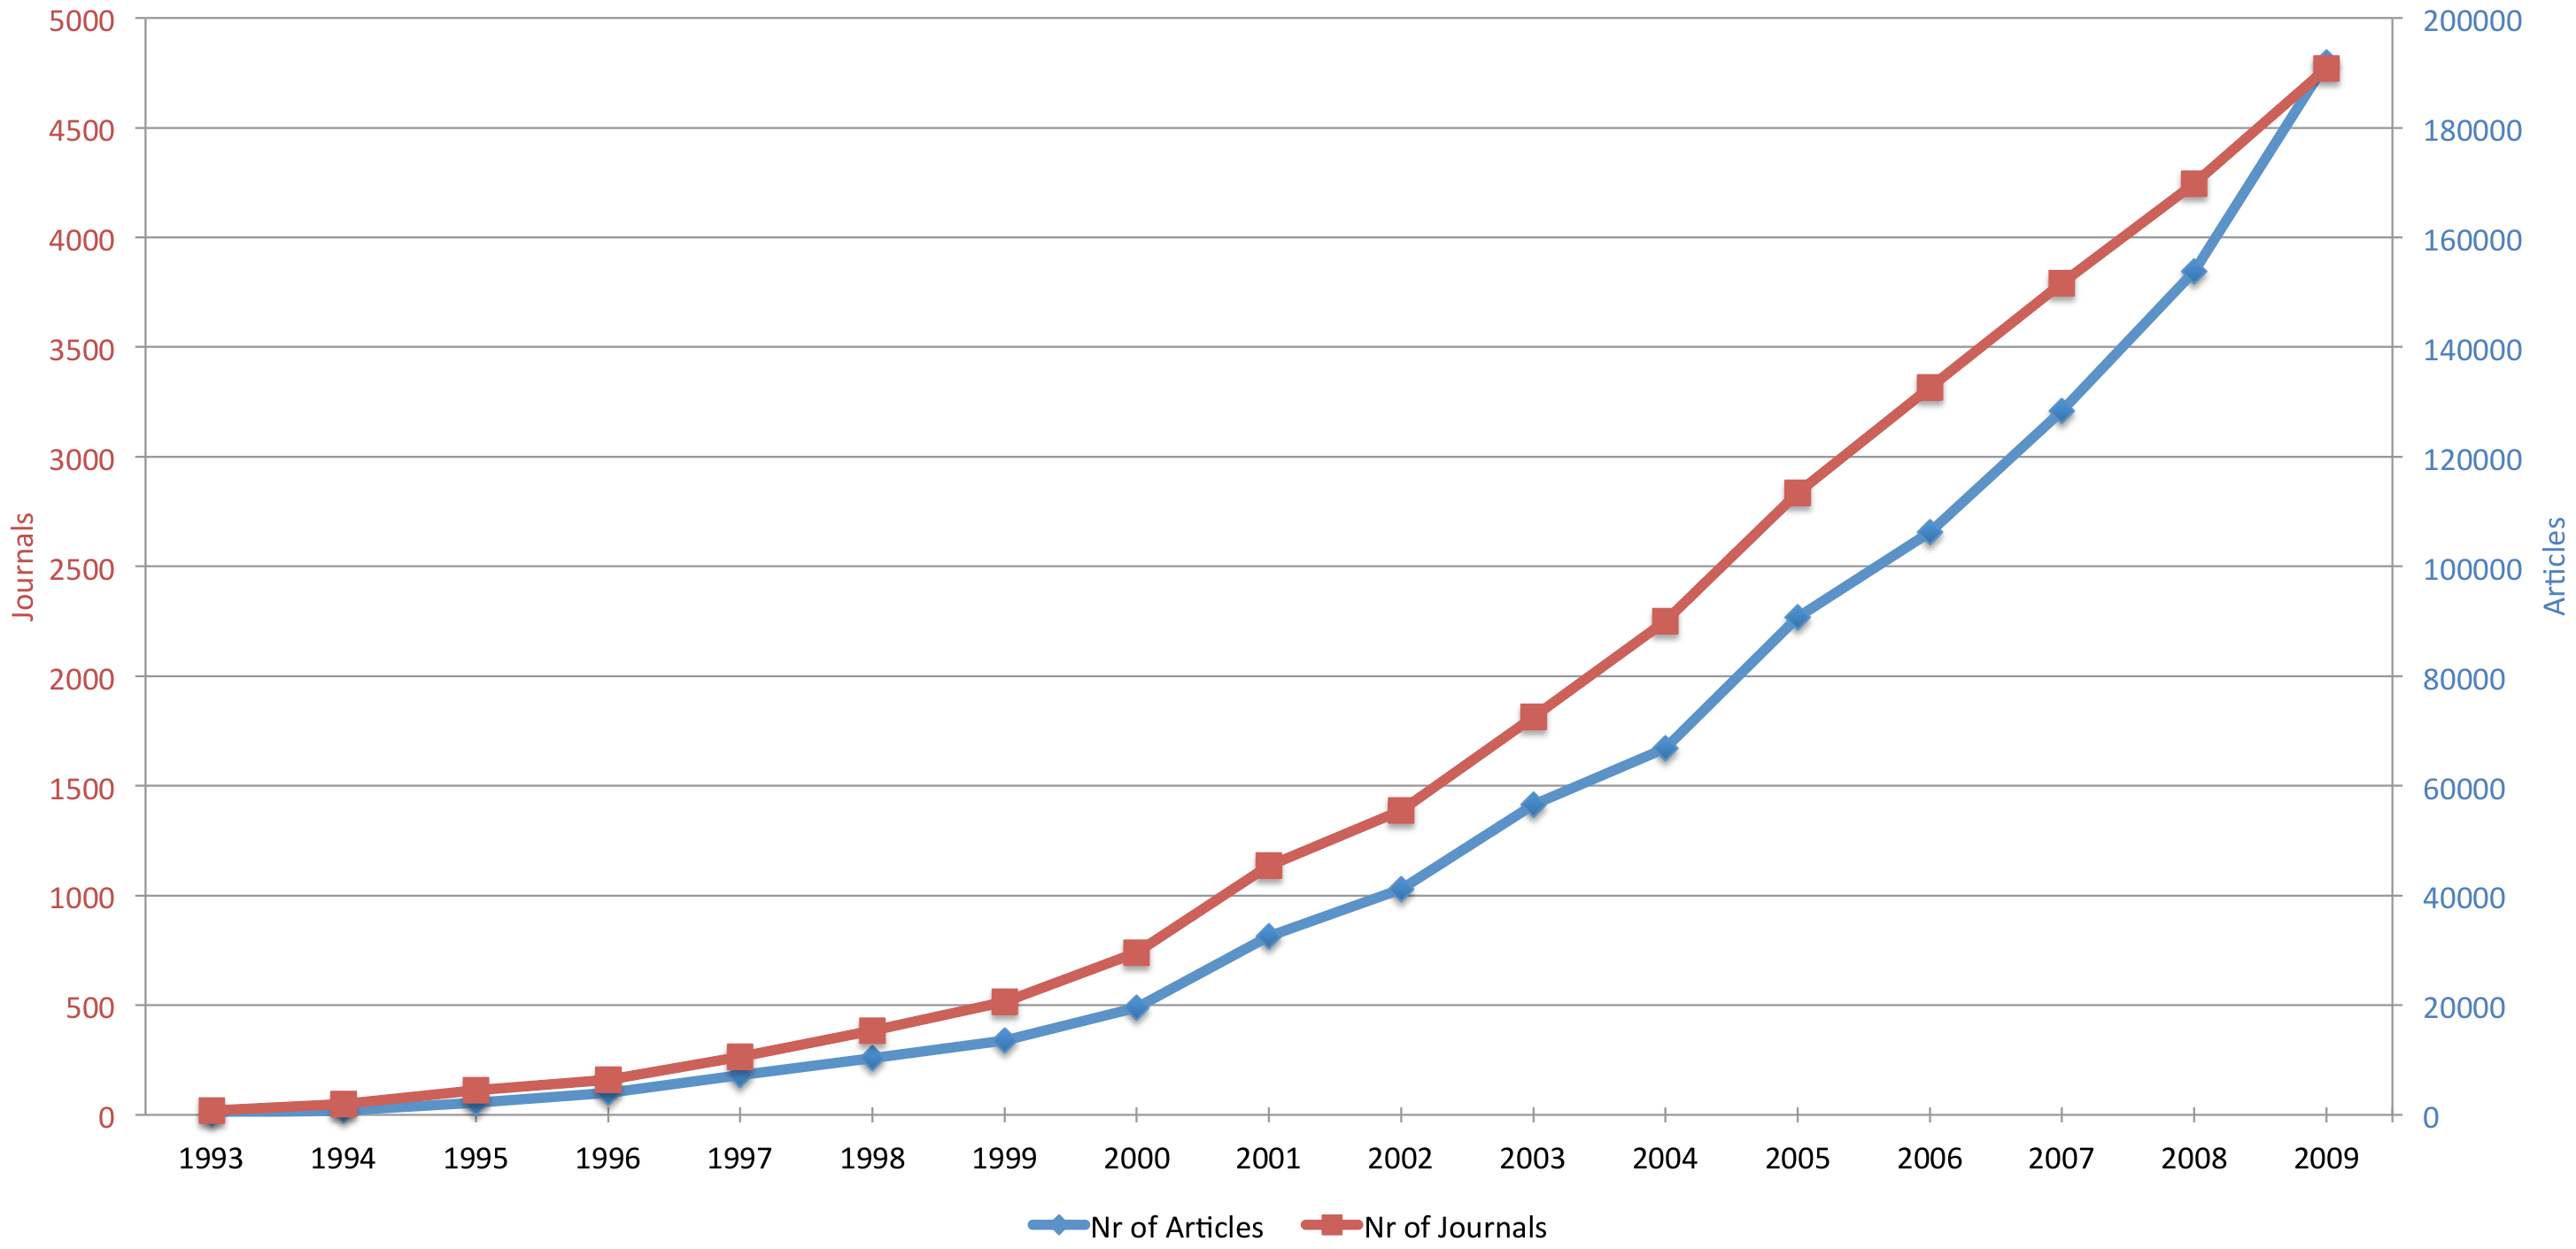
\includegraphics[width=\textwidth]{images/oa_increase}
    \end{centering}
    \caption{The growth of open access publishing between from 1993 to 2009 \cite{laakso2011development}}
    \label{fig:oa_increase}
\end{figure}

The total number of open access material is hard to estimate nowadays, but the
Directory of Open Access Journals (\url{https://doaj.org/}) measures the
amoung of open access journals world wide at 10 703 at the writing of this
thesis. The amount of open data journals and articles is growing faster than the amount
of more traditional, non open data journals \cite{laakso2011development}. This
is likely to correlate to the increased amount of open access mandates, since
mandatory open access rules imposed to the researchers correlate to a four
time increase in deposits to open access repositories
\cite{DBLP:journals/corr/SwanGHH15}.

For further reference, we can recommend the work of Stevan Harnad as a good
starting point to open access literature. He's referenced in
\cite{DBLP:journals/corr/abs-cs-0606079}, \cite{harnad2004comparing} and
\cite{harnad2004access}. If you are interested in data related to open access,
it's available botj on the Directory of Open Access Journals as well as in a
public data repository about hte growth of open access at
\url{http://dataverse.scholarsportal.info/dvn/dv/dgoa}.

\section{Research data open access publishing}
\label{sec:research_data_oa}

The idea to make research data openly accessible has been around for a long
time. As early as 1985 policies and practices to share reserach data to further
reserach and prevent fraud were developed \cite{fienberg1985sharing}.
The Internet and the emergence of data intesive science have changed the the
possibilties and quantities of research data. Research Data Alliance (RDA)
has been founded in 2013 to address the growing need of research data
publishing and sharing infrastructure \cite{DBLP:journals/dlib/BermanWW14}
\cite{DBLP:books/ms/4paradigm09}. Despite this, research data open access
publishing is far from research paper open access publishing.

Research papers should be self contained in the sense that a if you know the
area of research, you can read the research paper and understand what it was
after. Research papers often contain the processed results of the research data
behind them as well. Research data, however, is rarely self contained and
requires metadata to be useful for re use. It's also worth noting that datasets
nowadays will not be used solely by people who are experts in the fields that
the research data originated from nor will people work in geographically in the
same locations anymoer which makes metadata even more crucial for reusing the
data \cite{DBLP:journals/jbi/HarrisTTPGC09} \cite{DBLP:journals/jasis/Borgman12}.

While research papers generally follow an established structure and can easily
be published online in a PDF format, research data comes in many different
forms and flavors. For example, phylogenetic trees used in evolution
research look nothing like the brain images gathered in neuroimaging
research. This imposes a technical challenge to the solutions that
could be used to share research data - file formats are different, the
file size may be range anywhere from few hundred kilobytes to multiple
terabytes and because many fields don't share common practices on how to
manage their research data even seemingly similar datasets might be
incompatible between researchers \cite{whitlock2011data}
\cite{DBLP:journals/fini/PolineBGGHHHHKMPSAK12}.

As such, research data open access and publication is not prevalent in many
fields of science. The practices of data sharing vary a lot between fields and
even inside disciplines \cite{DBLP:journals/jasis/Borgman12}
\cite{cragin2010data}. This takes place even while all fields of science are
becoming more and more data intensive and many fields, such as psychology,
could reap great benefits from sharing research data
\cite{DBLP:books/ms/4paradigm09} \cite{wicherts2006poor}. The following
sections \ref{sec:research_data_challenges} and \ref{sec:research_data_benefits}
delve deeper into the benefits and challenges of sharing research data by
publishing it with the open access paradigm. A paper by P Arzberger et al.
\cite{DBLP:journals/datascience/ArzbergerSBBCLMUW04} summarizes these
challenges and benefits in an organizational level.

\section{Challenges of sharing reserach data}
\label{sec:research_data_challenges}

Sharing research data poses many challenges, some of them organizational and
managerial while others have to do with the nature of reserach data and the
culture surrounding them. The challenges are presented in more detail below
\cite{DBLP:journals/datascience/ArzbergerSBBCLMUW04}
\cite{tenopir2011data}

\begin{itemize}
    \item Technological issues - there is a lack of infrastructure to
          effectively publish and share reserach data
    \item Institutional and managerial issues - the principles of open access
          require tailoring for insitutions, since datasets, research funding
          and similar matters require local management
    \item Financial issues - managing research data archiving and publishing
          infrastructure requires continuous financial investment beyond the
          scope of implementation and publication of the reserach projects
          results
    \item Legal and policy issues - national and international law set
          limitations to sharing research data
    \item Cultural and behavioural issues - in the end, reserach data sharing
          comes down to the actions of the researchers generating the research
          data and if the culture for it does not exist and the behaviour is
          not encouraged, there will be no sharing of research data
\end{itemize}

These issues are higlighted in the questionnaire responses in
\cite{tenopir2011data} for reasons for not making their data not accessible
to public, shown in table \ref{table:reasons_not_sharing}

\begin{table}[h]
    \centering
    \caption{Reasons for not sharing research data, questionnaire with 1329
    respondents \cite{tenopir2011data}}
    \label{table:reasons_not_sharing}
    \begin{tabular}{| l | l | l |}
      \hline
      \textbf{Reason}                           & \textbf{Responses}    & \textbf{Percent} \\
      \hline
      \rowcolor{Gray}
      Insufficient time                         & 603                   & 53.6\% \\
      \hline
      Lack of Funding                           & 445                   & 39.6\% \\
      \hline
      \rowcolor{Gray}
      Do not Have Rights ro Make Data Public    & 271                   & 24.1\% \\
      \hline
      No Place to Put Data                      & 264                   & 23.5\% \\
      \hline
      \rowcolor{Gray}
      Lack of Standards                         & 222                   & 19.8\% \\
      \hline
      Sponsor does not Require                  & 196                   & 17.4\% \\
      \hline
      \rowcolor{Gray}
      Do not Need Data                          & 169                   & 15.0\% \\
      \hline
      Other Reasons For Data Not Available      & 164                   & 14.6\% \\
      \hline
      \rowcolor{Gray}
      Should not be Available                   & 162                   & 14.4\% \\
      \hline
    \end{tabular}
\end{table}

The Tenopir paper \cite{tenopir2011data} contains many more userful tables,
showing for example, that many researchers (56.1\%) either don't know or don't have
metadata stadards for their research data and data comes in many different
categories without even going to the soecifics in the fields of science.

Research data may be serious pricavy concern especially in fields such as
genomics or healthacre related research where reserach data could be connected
to the participants of the study. There is a tension between sharing relevant
and good quality data and protecting the privacy of the participants - more
detailed data provides for a more rich research, but allows for an easier
connection on to the participants \cite{kaye2012tension}. Work is being done
to facilitate safe and accurate sharing of data with privacy concerns. Both
codes of conduct and techonoligal solutions are required, especially since the
data will outlive the participants of the study and the privacy must be
preserved for the entirety of the data's lifetime
\cite{DBLP:journals/jam/NohCJ14a} \cite{knoppers2011towards}.

A more implementation level problem to sharing research data is the fact that
due to the legal issues or maybe the desire to work on your data before
publishing it means that reserach data should be able the be shared more
locally in addition to being open to the whole world. In practice, this means
that there should be means to provide access to the research data to
collaborating researchers or people within the research organization you are
working in to enable collaboration \cite{DBLP:journals/libt/Witt08}.

\iffalse
\subsection{Research data is diverse}

While research papers generally follow a
strict structure and can easily be published in a PDF format, research data
comes in all forms and flavors. For example, research data from a brain imaging
study will look completely different from a dataset that originates from
sociological research (citation). Not only the shape of the data is different,
the size of datasets can vary from the few megabyte survey results to the
multiple petabyte simulation results from a particle collider.

Even when you get down to practicalities the diversity of research data offers
challenges - results generated from one software might be binary incompatible
with another software within one field of science. And even if you were using
the same software, our versions might be different or you might do things in
such a different way that you are not compatible with other working on the
same field.

\subsection{Research data requires metadata}

Metadata refers to data about data. It's a rescription of the data and entails
details such as when was the dataset collected, what kind of equipement was
used or if there was something noteworthy in how the experiment was run
(citation). Due to the diversity of data in different fields, the metadata
differs between fields as well (citation). Some standards for metadata exist,
but not an all fields of science (citaiton).

Research data in and on itself is the most important thing to be published, but
working on someone else's research data without the relevant metadata adds
another layer of complexity and might mean that you cannot use the data at all
(citation). One reason to publish your data is to make reproduciton of you work
(citation) easier, and without proper metadata it is hard or impossible to
do that.

\subsection{Research data might be a privacy issue}

In many fields of science (healthcare, telecommunication to name a few) the
privacy of the participants to the studies is essential. If you go about
publishing your data, you need to be concious about maintaning the anonymity
of the people taking part in your research (citation).

\subsection{Research data might be published locally}

Due to privacty issues or maybe funding issues it might be so that the data
that is used in research cannot be published to the world but maybe you can
publish it within your orgnanization or upon request. This sets access rights
requirements to your dataset, so while you might be able to openly publish
your metadata in order to tell the world that your dataset exists, your dataset
should not be available for everyone (citation). 

\subsection{Research data requires support from higher ups and related partners}

Individuals can publish their data any way they wish as long as it's within
legal boundaries. However, if institutions such as universities or librareis
wish to venture into publishing their research, individual researchers and
people working with the data need support from their organizations. Studies
have shown (citation) that organizations need to commit to the idea of open
access publishing in order for it to work.

\fi

\section{Benefits of publishing research data}
\label{sec:research_data_benefits}

When talking about the benefits of publishing and sharing reserch data two big
points are generally made. Firstly it's thought that publishing and sharing
reserach data pushes science forward by enabling more people to work on the
data and subsequently accelerate the process of making relevant discoveries.
It's also not to be forgotten that reproducibility is one of the founding
pilalrs of scientific process and reqproducing others' work without access
to their data is very hard \cite{jasny2011again}.
Secondly it's thought that the publishing of research data makes your
research papers better, giving them credibility and yielding more citations in
the process. There are more subtle benefits as well that are discussed later
in this section.

Publishing research data benefits different stakeholders involved in the
data publishing game, as shown in figure \ref{fig:beneficaries}. The figure
also lays out how the rationales of sharing research data affect the different
stakeholder groups \cite{DBLP:journals/jasis/Borgman12}.

\begin{figure}
    \begin{centering}
        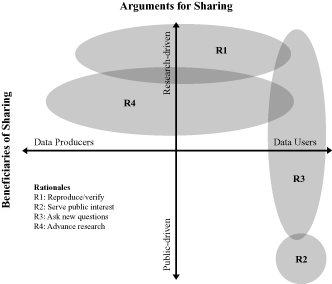
\includegraphics[width=\textwidth]{images/beneficaries}
    \end{centering}
    \caption{The different beneficiaries and rationales of data sharing \cite{DBLP:journals/jasis/Borgman12}}
    \label{fig:beneficaries}
\end{figure}

Publishing research data furthrers science by allowing new people to ask new
questions of the existing data \cite{whitlock2011data}, allowing for better
reproducability \cite{jasny2011again} and straight up widening the scope and
depth of the research in question \cite{DBLP:journals/see/FischerZ10}.
By making data publicly available the developers and people not included in the
scientific community, such as political decision makers, can also benefit from
the data being generated in the different fields of research
\cite{DBLP:journals/jasis/Borgman12}.

The benefits of research data publishing are not as straightforward as
publishing papers. Academic credit is distributed by the number of papers you
publish and by the number of citations you get to those papers. Research data
is often viewed as the fuel to the research. The actual downsides, from the
reserach, are covered in the next section (forward reference).

\subsection{Publishing reserach data yields more citations}

One of the most direct upsides of publishing reserach data is that it seems to
increase the citation count of the paper where the published data was related
to (citation). The research on this has not been done on all fields of science,
but the numbers from the fields it hase been conducted (medical science and
some others, put them down here at a later date) are impressive - up to
69\% (citation) increase in citation rates.

\subsection{Publishing research data makes your reserach reach more people}

While being quite intuitive, it's worth mentioning that open publishing of
research data results in your research being exposed to a larger audience
(citation).

\subsection{Publishing reserch data grows the impact of your research}

The impact of one's research is hard to quantify, but exposing more people to
your research and at the same time promoting your research papers enables your
research find places where it can make difference in the world (citation).
(this small section requires more meat on the bones)

\subsection{Publishing research data makes your research better quality}

The scientific principles require all scientific work to be replicateable. It
is quite hard to replicate your results just based on your paper, especially if
your paper is heavy on analysis dependant on your data (citations). In this
light publishing your research data in fact makes your research better quality.

Publishing research data should make all research data better as well. The
logic behind this is that if all research data was public, it would fall under
public scrutiny making it harder to publish fraudulent results and it would
force the authors of the data to make it more readable to the wider audience
(citation).

\subsection{Publishing research data can save you from fraud accusitions}

In addition to preventing fraud from others, if your data is public you could
easily deal with fraud accusitions by pointing people to your public data and
the analysis that was performed on that data (citation).

\section{The disadvantages of publishing research data}

There are a few strikes agains publishing research data. Some of the
disadvantages are more perceived than real, but they prevent the publication
of research data just as well.

\subsection{Preparing research data requires work}

As mentioned in section (reference backwards), publishing research data
requires metadata. Metadata entails good documentation as well as annotated
datasets and such that are not necessarily required during the research
project. Time taken away from researchers core work is a hindarance in their
daily work (citation).

This problem is made bigger by the fact that there are no best practices or
widely adopted tools to manage your data during your research process and
finally publish your data (citation).

\subsection{Publishing research data adds costs to the publication process}

Publishing is not free from the financial standpoint either. Since sicentists
are not metadata experts nor are they experts in electronic publishing, other
facets of the research institution. Open publishing of research data requires
curators for the data (for example, from a library) and adminstrators for the
system that manage the reseatch data (citation). While these groups may have
communicated in the past to some extent, publishing research data is an effort
that requires a new kind of communication and collaboration within these groups
(citation).

\section[Validity of the benefit research]{Research on the validity of increased citation rate with publishing
research data}

There is also research that suggests that the increased citation rate shown in
studies is actually a statistical artefact and that research data publication
wouldn't have a direct correlation to the increased citation rate (citations).
There are not many of these papers, but their existense suggests that there
should be more critical studies to validate the benefits of open data
publishing. On the other hand, the amount of research data being published
is quite small copmared to all data that is being generated (citation), so
when more data becomes available this kind of analysis also becomes more
valuable and accurate.

\section{Research data sharing currently}

Research data sharing is being inpmplemented in different places nowadays on
different levels. Most relevant places for scientific data publishing are the
institutional repositories that are managed by research institutions and
different international and national organizations (such as EUDAT and
different discipline focused repositories).

\subsection{Insitutional data repositories}

Notes about institutional respositories (some citations are below)

\subsection{International repositories}

Notes about international repositories (also showing some, sucg as EUDAT)

\subsection{National repositories}

Could present CSC and the national library here at this stage.

\subsection{Requirements for data sharing}

Many funding bodies require researchers to publish resedarch data in addition
to the actual papers. The research shows, however, that even though publishing
research data is required, it is not being done in practice (citation). Even
papers that are considered high impact and fields that would benefit the most
from sharing data (such as psychology) do not share their research data
(citation).

\section{Adherence to data publishing requirements}

Many funding bodies and journals require the publication of research data
related to the research papers. Adherence to this requirement has been studied
and the results are that despite the demand for sharing research data it's not
being shared commonly. In one study 10 datasets were requested from a journal
that explicitly requests sharing datasets and only one dataset was received
\cite{savage2009empirical}. In a bigger study the authors were able to gain
63 datasets out of 249 possible datasets from a journal that also requires
datasets to be shared for reanalysis \cite{wicherts2006poor}. In a study of
500 hundred papers, of which 149 were not subject to any research data
publishing requirements, only 47 papers had submitted the complete raw data
online. Of the 149 who were not required to do publish research data did not
publish anything \cite{alsheikh2011public}. The 500 hundred papers in the last
study were selected from 50 different journals by selecting the 10 research
papers with the highest impact factor.

The reasons behind not sharing data were different. In the smallest study (\cite{savage2009empirical}),
where the reserachers were able to contact the people who refused the reasons
for not sharing are listed below.

\begin{itemize}
    \item Two email addresses listed on the original research paper were no
          longer valid and once one of them was reached she was on maternity
          leave and couldn't help
    \item Two of those who didn't share didn't give a reason for not sharing - on further
          inquiry one of them responded that he was not aware of the research
          data publishing requirements
    \item One stated that he was too busy and compiling the research data
          would be too much work
    \item One had changed institutions and no longer had jurisdiction over the
          data and the people in the publishing institution responded that
          sharing would have been too much work
    \item Three did not answer the inquiry at all at first - on further inquiry
          one of them replied that he was in favor of sharing data in general
          but wanted to conduct more research on the research data himself
          first
\end{itemize}

In the biggest study the authors postulated that factors such as the 6-12
months between the publishing of the papers and the authors' investigation
the reserach data publication policies might have changed, though this is noted
to be unlikely \cite{alsheikh2011public}.

\section{Sharing Big Data}

Big Data is generally defined by the three Vs - volume, velocity and variety.
Volume refers to the amount of data - there are not usually set in stone
metrics for the volume, but as rule of thumb one should consider a warehouse
full of computers as one computing unit when it comes down to big data.
Velocity means the speed that data is being gathered. Variety in the context
of big data refers to the fact that since big data usually comes from a variety
of sources, also the content and the format of the data varies. (citations)

Nowadays big data has an added V in veracity, which means the uncertainity of
the data. In the case of big data it's impossible to tell how much of your data
is reliable, since you typically don't do validation or vetting of our data.
(citations)

All big data instances don't of course contain all of the Vs. Big Data as a
concept is rather fuzzily defined, but all big data systems contain some of the
traits described above.

In this context sharing big research data adds additional challenges, since 
you can't simply download big data research files to your computer. Some
research has gone to sharing big data datasets (cite), but since there is a lot
of work left to make "small" data sharing and management work this thesis
focuses on more traditional research data sharing.

\section{Sharing research workflows}

In addition to sharing research data, research has been done in sharing
reserch workflows. Sharing research data workflows makes replicating
experiments and sharing results even easier. Sharing workflows is common in
fields where collecting data and doing analysis are easy to automate end to
end, such as genomics (citations). This thesis does not focus sharing research
data workflows, but using making the process behind the results more visible
should make scientific work better. 

\section{Some technical examples of repository software}

\subsection{Dataverse}

\subsection{Hydra}

\subsection{CKAN}

\subsection{iRODS}

\section{Interesting research data related literature}

\section{General points}

Points to touch on this section:

\begin{itemize}
    \item sharing data and open publishing of results has been studied
    \item generally it's noted that sharing papers online leads to benefits
    \begin{itemize}
        \item citation rate increases
        \item impact of your research grows
        \item you reach wider audience
    \end{itemize}
    \item some research contradicts the increase in citation (comparing open
          access and closed citation), claiming that the increased citation
          rate of open access things is a statistical artefact
    \item in addition, there are papers on how you should organize your data
          sharing ways
    \item funding bodies have started demanding the publication of data
    \begin{itemize}
        \item however, people who have published in papers that require you
              to publish data don't actually do that
        \item publishing data is rare even on fields where sharing would be
              great
    \end{itemize}
    \item privacy and security is a concern
    \item present some systems available
    \item some technologies and platforms could be mentioned
    \begin{itemize}
        \item iRODS
        \item CKAN
        \item genomics sharing platforms
    \end{itemize}
    \item and then there are fringe cases related
    \begin{itemize}
        \item Adam
        \item Galaxy + Hadoop integration
    \end{itemize}
    \item notes about big data (paper about the difficulties of big data in
          research infrastructure
\end{itemize}

Article \cite{piwowar2007sharing} discusses how open data increases citation
rate.

Article \cite{howison2005ossmole} is about a collaborative repository.

Article \cite{savage2009empirical} tried requresting data from authors who were
obligated by the publisher to publish data, but 9/10 did not share data.

Article \cite{piwowar2011shares} discusses low and slowly growing publishing
rates even on fields where publishing would be most advantageous.

Article \cite{tenopir2011data} discussed the culture and perceptions of
research data publications, showing that the culture is not well developed
and organizations don't support  researchers in their long term data storing
needs.

Article \cite{whitlock2011data} discusses best practices and such and so.
Gotta read more carefully when I'm on Aalto network.

Article \cite{wicherts2006poor} shows poor availability of data even though
they should be available.

Article \cite{alsheikh2011public} shows that even high impact papers (define
high impact later) subject to data publishing requirements don't necessarily
publish stuff. Those not subjected to any policy don't publish anything.

Article \cite{piwowar2011data} promotes good ROI on publishing research data.

Article \cite{hrynaszkiewicz2010preparing} shows some guidelines for sharing
data and stuff.

Article \cite{DBLP:journals/jasis/Borgman12} tackles the conundrum of research
data.

Article \cite{DBLP:conf/isiwi/AlamMS15} discusses an easy to use platform for
sharing data.

Article \cite{DBLP:conf/jcdl/SimonGSG15} describes a video sharing tool for research
use.

Article \cite{DBLP:journals/dlib/BermanWW14} describes RDA (research data
alliance), as a entity that promotes research data sharing.

Article \cite{DBLP:journals/jam/NohCJ14a} describes a method to encrypt private
information on a public platform.

Article \cite{DBLP:conf/ACMdis/CurmiFW14a} sharing data in social media
(biometric data), read more carefully.

Article \cite{DBLP:conf/esws/EkaputraSSB14} describes and ontology based
system for sharing research data.

Article \cite{DBLP:journals/ijdc/DoornDH13} discusses whether open publishing
of data could prevent scientific fraud following a hude fraud incident.

Article \cite{DBLP:journals/ijdc/GrootveldE12} pilots the idea of a research
data peer review.

Article \cite{wicherts2011willingness} examines if not publishing research data
means that results are in fact weaker.

Book \cite{DBLP:series/synthesis/2010Rajasekar} is the iRODS primer, cite
on.

Data intensive science (the fourth paradigm), \cite{DBLP:books/ms/4paradigm09},
things to cite regarding the data science.

CKAN platform investigation, \cite{winn2013open}.

Article \cite{DBLP:journals/fini/PolineBGGHHHHKMPSAK12} talks about sharing
data in the field of brain imaging (also tackles general issued in the sharing
field).

Article \cite{knoppers2011towards} outlines code of conduct for international
data sharing in the context of genomics.

Article \cite{cragin2010data} tackles issues in insitutional and other small
institutions.

Article \cite{DBLP:journals/fgcs/RoureGS09} is about sharing scientific
workflows.

Article \cite{kaye2012tension} is about privacy issues and how to share
healthcare data in good fashion.

Classic free lunch is over (\cite{sutter2005free}), need for concurrency
increases and at the same time computing power becomes more expensive and
storage cheaper.

Article \cite{DBLP:conf/cloudcom/DemchenkoZGWL12} discusses tha challenges
of big data infrastructure in the scientific research facilities.

Article \cite{hjorland2014curating} tackles the role of libraries and data
handling professionals in the electronic world.

Executable papers as a method to reproduce data, refer to something like
this \cite{DBLP:journals/procedia/GorpM11}.

From the good old days there is this book,advocating research data sharing
before it was cool \cite{fienberg1985sharing}.

Gathering data automatically, metadata drive and so on
\cite{DBLP:journals/jbi/HarrisTTPGC09}.

Institutional repository stuff, distributed environment (university related),
here \cite{DBLP:journals/libt/Witt08}.

User engagement required in order to make data curation success with
researchers, see here \cite{DBLP:conf/ercimdl/Martinez-UribeM09}.

Overview about who shares, what, how and so on, see
\cite{borgman2010research}.

Role of libraries in emerging e-science (libraries should curate data, they are
data management experts), \cite{heidorn2011emerging}.

Good and bad things (perceptions too) about sharing research data. Medical
field, South Africa \cite{denny2015developing}.

Time is right for repositories and sharing data (data is growing, how are you
going to handle it?), see \cite{lynch2008big}.

Article \cite{eysenbach2006citation} talks about the citation advantage you get
from publishing in an open access way.

Article \cite{DBLP:journals/oir/XiaN12} talks more about getting more citations
by publishing open access style.

Article \cite{antelman2004open} is more praise towards open publishing and
research impact.

Article \cite{lawrence2001free} is an oldie, but has a lot of citations and
does talk about the merits of free online access.

Article \cite{DBLP:journals/joi/CraigPMPA07} talks about the bias of open
access - maybe it does not actually get you anywhere. Important to bring out
opposing views - it's not all rosy in the world of open access.

Article \cite{davis2008open} is another opposing voice towards the gains of
open publishing, stating that you might reach a wider audience with open
publishing but increased citation rates might be an artefact from other
sources.

Adam article \cite{DBLP:conf/sigmod/NothaftMDZLYKAH15} would be interesing from
both big data and automatic data collection. All data is data intensive
science, so making a platform to handle those aspects is interesting.

Article \cite{cimino2010clinical} speaks about a data repository implemented
by the US National Insitutes of Health where you can get health data.

Article \cite{bax2006development} presents a free meta analysis tool for health
sciences. Possibly interesting from the point of view of analyzing data
collected from multiple sources.

Article \cite{DBLP:conf/bcb/PiredduLSZ14} shows a data oriented workflow
system. Big data, genomics analysis and workflows.

As an example of repository within a field (genomics, this time), this paper
\cite{craigon2004nascarrays} shows a system to store and share data related
to this field. Another similar system here \cite{DBLP:journals/nar/EdgarDL03}.

Collaboration and sharing is presented in paper \cite{craigon2004nascarrays} in
the context of distributed open source development.

Some words about an institutional repository \cite{gibbons2009benefits}, also
quite cleanly summarizes the considerations that come in when thinking of
deploying an institutional repository.

Article \cite{DBLP:conf/icegov/SayogoP11} is yet another paper describing
the detriments to scientific data sharing.

Article \cite{irodsinproceedings} is the thing Jyväskylä wrote about the iRods
native cross GUI client.

Article \cite{DBLP:conf/elpub/Hedlund08} is about gouging the attitudes of
business people towards open publishing.

Article \cite{laakso2011development} talks about the evolution of open
publishing at the age of the internet, and points out that open publishing
is of course become more common and cheaper with internet.

Article \cite{suber2007open} is a short overview of open access publishing.

Article \cite{harnad2004comparing} boasts a bigger amount of citations to
papers that are openly accessible to the papers that are not (published in the
same journals even).

Article \cite{bailey2008open} is a nice summary about what is open access.

Article \cite{DBLP:journals/corr/abs-cs-0606079} is a longe study about OA
advantage.


\startchapright\chapter{Positioning the Thesis}
\label{chapter:positioning}

Master's theses don't live in a vacuum. To position the thesis and provide the
best possible outcome for Aalto University we made an effort to find out what
is the current state of research data publishing and sharing as well as what
are the current challenges and projects in the Finnish landscape. While the
literature review in Section \ref{chapter:background} covered the overall view
of the current status of publishing and sharing research data and research
papers, the goal of this thesis is to provide value in the context of Finland.
The tools used to position the thesis were interviews, benchmarking existing
solutions and a questionnaire.

\section{Researcher interviews}
\label{sec:expert_interviews}

Scientists and researchers are the core user group of any publishing or sharing
system since they are the ones generating the data to the system and populating
the system. The research also shows that a successful repository system requires
user engagement \cite{DBLP:conf/ercimdl/Martinez-UribeM09}. Scientist and
researcher interviews were conducted within different research groups and
researcher in Aalto Otaniemi campus. The goal of these interviews was to learn
how data management is taught and used in Aalto University and what are the
scientist and researchers perceptions on sharing and publishing research data.
Previous experiences with sharing and using others' data were also gathered.

In an interview with a research group\footnote{M. Nurmela and the Complex
Networks group at Aalto University, \url{http://becs.aalto.fi/en/research/complex\_networks},
personal communication, July 31st, 2015} the findings fell in line with the
findings from literature. As of writing of this thesis, data management is not
systematically taught for the researchers and
there is no culture or experience in data sharing. Upon questioning it became
clear that the data in the possession of the researchers would have required
a lot of cleaning and metadata additions prior to publishing - this is no surprise
considering the fact that the datasets they were using were not designed to
go public in the first place. Though lack of metadata practices and lack of
publishing infrastructure were also brought up.

Some members of the research group had shared some of their datasets through
public cloud services such as Google Drive\footnote{\url{http://drive.google.com/}}
with collaborators and used others' datasets. This also raised the point that
in order to use others' datasets they had been asked to cite the papers that
used that dataset, underlining the the undeveloped culture of research data
sharing. Some members of the group saw big advantages in making research output
public, especially from the angle of reproducability, but also raised concerns
about the privacy issues that for example telecommunication data would cause.
The members of the group were also concerned about about the size of their
data, since using the existing solutions to share hundreds of gigabytes worth
of datawould prove cumbersome.

One member of the group had taken a role of a mentor with the data management
issues, teaching the others to use databases and version control software to
handle their data and code. The other members of the group, interviewed
separately, noted that an effort had been made towards better policies in data
handling. The group pointed out that personalized assistance and word of mouth
were an efficient way to learn "boring" things like data management. Own
previous experience and learning by doing seemed to be the main way people had
learned to, for example, comment their code or arrange their research data into
databases so that accessing them would require less time and managing code
would be easier.

Discussions with the complex networks groups also brought up the point that
even though some data could be published for all the world to see, some data
should be only accessible to people within Aalto University and some should
even have a more fine grained access control set to them.

In a separate interview with a brain image researcher\footnote{M. Nurmela and
E. Glerean, personal communication, August 13th, 2015} similar concerns arose.
Brain imaging data is large and that makes sharing it hard. Brain images are
also considered personal data and publishing them is problematic. The
researcher expressed interest in sharing and using others' datasets, but
lacked the tools to do so.

\iffalse
\section{Scientists}

Scientists would be the main user or stakeholder that would use the system. It
is important that a system that would help them store and publish research data
would provide value for them without being another system that is a huge
annoyance to use.

\subsection{The goal of the interviews}

It is interesting as to what is the current status of research data management
and how research data is being published. Also what was learned in interviews 
with other stakeholders it became clear that research data management covers
much more than just the publishing part, so it was important to find out
whether the scientists were actually being trained to handle research data.

The secondary goal is also to gain input on how the system to manage and
publish research data should look like if it were to be implemented.

\subsection{Results of the interviews}

\fi

\section{Science IT staff}
\label{sec:sci_it}

If a system to publish and share research data would come to be it would have
to be maintained and run by people other than the researchers, since the job of
the researchers is to do research and not maintain software systems. With this
in mind the people managing the scientific IT systems are a key component to
building a successful research data management, publication and sharing
platform.

In interviews with a scientific IT systems specialist\footnote{M. Nurmela and
M. Hakala, personal communication, July 1st and 7th, 2015} the findings again
aligned with the findings from literature. There is a lack of metadata
standards that would make data storage and management uniform across
institutions and disciplines. Finland has projects going on related to open
science\footnote{\url{http://avointiede.fi/}} and CSC\footnote{\url{https://www.csc.fi/}} is
building scientific computing environments for Finnish institutions (research,
library, archival, education and such). According to the specialist
collaborating with all these ongoing projects would benefit both parties and
also allow Alto University to develop systems that are not just point
solutions. This would also make sense from a financial point and practical
point of view, since research is nowadays done in collaboration with other
institutions and working together would enable that.

From the point of view of IT system specialist the ideal system for research
data includes the whole lifecycle of the data. This entails education on how
to manage the data from the creation to the publishing and infrastructure that
can be tailored to fit the different user needs. Research data is comes in
many forms so a solution that is not flexible would be unsuitable.

University of Jyväskylä has implemented a data repository system\footnote{\url{https://dvn.jyu.fi/dvn/}}
as well as an iRODS\footnote{\url{http://irods.org/}} system to manage and
store research data. In an interview\footnote{M. Nurmela, I. Korhonen and A.
Auer, personal communication, August 19th, 2015} they noted that nowadays
universities need a platform to publish research data. Jyväskylä is among the
first in Finland to implement a data policy in practice, offering an
infrastructure to manage data during the research projects and publish the
results in the end (even though Dataverse and iRODS are not currently
easily compatible with each other, though some work has been done for
that\footnote{\url{https://irods.org/wp-content/uploads/2014/06/Odum-DFC-iRODS-Boston.pdf}}).
They are also working with CSC to get their iRODS system talking with the iRODS
system at CSC.

The Jyväskylä experts told that while the Dataverse system was easy to install
and modify to accept Jyväskylä University credentials, it still had a long way to go
before it was universally accepted within the university. At the time of
writing this, the Jyväskylä Dataverse has been running for approximately a
year and it contains a very small amout of datasets. Some research groups,
however, are using it manage their internal datasets. As to how to get the
more datasets into the system, they planned to continue educating about it
and making it that way a part of researchers' routine.

Jyväskylä was more involved in development of the iRODS system, having even
developed a system to facilitate collaboration between researchers
\cite{irodsinproceedings}. The Kanki system is a desktop interface to the iRODS
system that allows users to easily access and modify data stored in the iRODS
data grid. The Kanki system is not about publishing research data but data
management during a research project. iRODS also has federation capabilities,
meaning that two iRODS instances could be integrated such that you could
access the data from the other system. When writing this Jyväskylä and CSC
were planning to start testing the federation capabilities. Following up on that
on a later date would be interesting.

\iffalse
If there was to be a system to manage and publish research data, it would have
to be maintained by someone. The obvious answer is to go to the administrators
of institutional software infrastructure.

\subsection{The goal of the interviews}

What is the stance of the administrative side on a data repository? How does it
fit the role of the infrastructure administrators? Building software systems is
not only about what people want and what existing systems prove to be the best,
human factors and elements like funding affect these decisions.

At least in Aalto the staff maintaining the infrastructure are also aware about
who are the people hosting research data on school infrastructure, making them
also knowledgeable on how things are handled right now.

\subsection{Results of the interviews}

\fi

\section{Project managers on research data related systems}

Building and running software systems requires commitment not only from the
primary users discussed in Sections \ref{sec:expert_interviews} and
\ref{sec:sci_it} but the management that supports them. The priorities of the
managerial types might not lie in the usability or maintainability of the
system, but rather in managing costs and minimizing risks.

From Aalto side the desire is to minimize the systems we have to build and
maintain ourselves - since CSC exists to provide scientific computing and
storage resources, why should we not use them? Non established or new fields
of science could have value from a local repository, but those that have
international or discipline specific repositories could use those as well.\footnote{M. Nurmela, A. Sunikka, personal communication, July 17th, 2015}
Certainly managing research data is a problem and a consensus solution has not
emerged.

The Finnish National library is in charge of long term preservation of relevant
objects in the Finnish research. They are building a long term storage
solution\footnote{\url{http://avointiede.fi/tutkimus-pas}}, data management
plan tool\footnote{\sloppy\url{http://portti.avointiede.fi/tutkimusdata/tuuli-tyokalu-tutkimuksen-datanhallinnan-suunnitteluun}} and managing the Finnish unique identifier
service\footnote{\url{http://www.kansalliskirjasto.fi/fi/julkaisuala/urn.html}}.
They also manage a Finnish cultural repository\footnote{\url{https://www.finna.fi/}}.

The most important thing to for the project manager at the National Library
was that metadata associated with the data has to be good - otherwise
archival, management and reuse is impossible. Making metadata work within an
institution requires commitment from all levels of management and tools to
facilitate that. It is also important to note that even if two systems within
different organizations would be technologically perfectly compatible,
the bottlenecks might stem from different policies in different organizations
and the bureaucracy that comes with it. This thought lessens the burden for all
technology to be perfectly compatible.\footnote{M. Nurmela and E. Keskitalo, personal communication, August 21st, 2015}

\iffalse
Implementation and running of different systems related to research data
management and publishing are being implemented and developed around Finnish
institutions. While people working on and with these systems were included in
the previous two sections (backwards reference) there are people who are in
charge of those systems and make the decisions on which to purchase.

\subsection{The goal of the interviews}

Systems that have to do with entities as big as universities or even nations
need management and getting a view from only the people using them is not
sufficient when designing such a system. People in managerial positions have
different objectives and needs for a system like this.

From people in positions like this it is important to learn about the bigger
picture. When dealing with a concept like sharing research data it makes sense
to try make systems talk to each other and not everyone to implement their own
system in their own silo.

\subsection{Results of the interviews}

\fi

\section{Librarians}

Publishing research data requires expertise in digital publishing and metadata
experience. University libraries are experienced in publishing digital reserach
papers (open access or restricted access) and making metadata descriptions
about digital and physical publications. This makes librarians and libraries
and essential part in bringing research data to the open publishing world.

In an interview with the people responsible of the digital publishing at Aalto
University Library\footnote{M. Nurmela and A. Rousi, personal
communication, September 30th, 2015} brought up the essential role of
librarians as the classifiers and describers of the data. Professional data
handlers can do very good metadata descriptions, even if they are missing
some of the domain knowledge related to the research data. The librarians
also handle the relationships to the publishers - though what is the role
of traditional science publisher authorities in the future when organizations
can publish datasets and even research papers papers easily on their own.

Aalto University library runs the Aaltodoc service\footnote{\url{https://aaltodoc.aalto.fi/}}
which contains full text materials on research papers and theses published
in Aalto University. The system runs on on DSpace\footnote{\url{http://www.dspace.org/}},
an institutional repository software for publishing digital objects. DSpace
focuses on publishing research papers, but the person in charge of the system
reckoned that it probably could be modified to host small datasets as well.
This would require some additional work of course, so a better way could be to
link the research papers the relevant datasets in the corresponding systems.\footnote{M.
Nurmela and J. Nevala, personal communication, August 27th, 2015}

The National Library of Finland is in charge of implementing long term storage
and archival of important datasets and other research material. From that point
of view and also research data in general the biggest challenges are not
technical - software systems to store data and manage it exist, but making it
so that institutions themselves commit to managing and storing data is the
bigger challenge. And once different institutions are able to manage their own
data, the collaboration between the institutions' systems is likely to be
more difficult in the policy and bureucracy sense. There are also many
unresolved questions related to long term storage. Who decides what datasets
are used for the long term storage? What kind of metadata long term storage
requires in addition to the metadata already in the original dataset? The work
to figure out these things and the Finnish long term archival project is going
on during the writing of this thesis.\footnote{M. Nurmela and E. Keskitalo, personal communication, August 21st, 2015}

\iffalse
Librarians are metadata experts. They are trained to describe scientific
content, manage and sort that content and nowadays they also work with digital
publishing. In some libraries across the globe (citation) the libraries have
taken responsibility of also publishing research data.

\subsection{The goal of the interviews}

What is the current status of digital publishing in Finland? And how do the
libraries themselves see their role when publishing research data enters the
equation. How should we organize the collaboration between libraries and
scientists?

\subsection{Results of the interviews}

\fi

\section{People organizing courses}

Teaching is another role within the university that would benefit from the fact
that research data would be readily available for the students to consume and
run analysis on. If we wanted to make research data management an integral part
of scientists' daily routine it would have to be integrated to the teaching
regime taught in schools.

\subsection{The goal of the interviews}

Aalto University has a minor in Data Science, but does it have any means to
support that? How is data science and in its wake data management taught
currently in the university?

\subsection{Results of the interviews}

\section{Representatives from CSC}

CSC offers an interesting angle to the research data management problem. CSC
offers nationwide computing services and they should have a role in sharing and
managing research data.

\subsection{The goal of the interviews}

CSC must have some plans and current ideas on how to manage and share research
data since the world is moving towards publishing research data. It also makes
sense from their point of view to offer both computing power and storage
services and it would be interesting to know what are their plans in that
sector and if they do not have plans what is going on with that.

\subsection{Results of the interviews}

\begin{itemize}
    \item many experts
        \begin{itemize}
            \item scientists
            \item science IT staff
            \item people in charge of policies and development of university
                  systems
            \item developers in libraries
            \item library representatives
            \item project managers at CSC (in charge of nationwide computing
                  services)
        \end{itemize}
        \item fill in input from each once it's time to write those
        \item notable common findings
        \begin{itemize}
            \item metadata management is a huge problem
         demand to publish research data   \item no education, tools or any idea on how to work with that
            \item no experience in data sharing
            \item not willing to use lots of time for metadata management
            \item the university would prefer not to store their own
                  datasets, but would rather work with other places
            \item library should have a role in managing metadata and coaching
                  the scientist with their dataset management
            \item data intensive science is being taught in Aalto, but without
                  own infrastructure
        \end{itemize}
        \item also a common conclusion here is that there is not consensus
              within Finland on how to arrange ourselves with research data
        \item there is the nationwide computing service provider, CSC, but
              there is no common push towards data repository or managing
              research data
\end{itemize}

\section{Data management questionnaire}
\label{sec:questionnaire}

A study was conducted in Aalto University about data management. The goal of
the study was to find out the current needs as well as the current status of
research data management within Aalto University (TODO: figure out a good way
to cite this study). 87 people submitted answers to the study from all the
schools in Aalto. The breakdown of answers is shown in figure (reference to the
figure).

The study outlined the challenges within Aalto University. The answers asked
most for services in storing data, metadata, finding data, archiving, sharing
and backing up data. The challenges where the requirements span from are both
technological and policy related. In the list below the the answers are
compiled by percentages:

\begin{itemize}
    \item The name of the folder/file or the location of the folder/file is
          forgotten or poorly described, approx. 35\%.
    \item Ownership of the data, approx. 30\%.
    \item Not enough disk space, approx. 30\%.
    \item Version control, approx. 30\%.
    \item Non functional or corrupted equipment, 29\%.
    \item Sharing data with partners and collaborators, 24\%.
    \item Unwanted deletion of data, 22\%.
    \item Complicated user interface, approx. 20\%.
    \item Forgetting password, 17\%.
    \item Access rights, approx. 12\%.
    \item Failed backup, 8\%.
\end{itemize}

The study shows that there are indeed a need already in place for a system to
manage research data in Aalto as well as training and policies to support data
management through the lifecycle of data.

\section{Benchmarking existing solutions}
\label{sec:benchmarking}

Technical solutions to publishing and managing research data exist already, many
of them open source and free. Some of the solutions were mentioned in the
literature review in section \ref{sec:implementations_literature}. This section describes
those systems and some other in more practical detail.

\subsection{Harvard Dataverse}

\subsection{Hydra project}

\subsection{iRODS}

\subsection{CKAN}

\subsection{Invenio and Zenodo}

\subsection{GitHub}

\section{Work that is currently going on in Finland}
\label{sec:finland_current}

Here we are going to paraphrase research and interesting things going on in
Finland at the moment. Items to look into would be:

\begin{itemize}
    \item IDA and Etsin services by CSC
    \item the ATT initiative going on
    \item the social science library by Tampere University
    \item the long term storage developed by national library
    \item national library also develops the URN schemes
\end{itemize}

A question to ask Keijo later is that many of the people interviewed told about
their upcoming research. Is it interesting here or should we stick to things
that exist for sure?

\section{Outcomes of the positioning research}
\label{sec:positioning_outcomes}

Here we will describe what we learned about the positioning of the work.

First of all, it is clear that the research data management is not jut a
technical problem. Perfectly fine technical solutions to the problems of
publishing research data and managing your data in a safe way exist but the
real problem is to get people and organizations to use them.

Research data management questions transcend the university level as well
as the national borders. After all, the goal of publishing and sharing
research data is to make science move forward in a faster clip and make the
quality of research better by collaboration - ergo there is no point in every
institution in Finland to manage their own research data repositories and
archives.

With this in mind this thesis focuses on providing a prototype solution that
serves as a wireframe for implementation that should be done in such a way that
all institutions in Finland would benefit from that. In addition this research
will provide a road map style solution that would make use of existing know-how
and work and serve as a possible proposal on how to bring research data
management into all Finnish institutions that need that kind of service.


\startchapright\chapter{Prototype Solution}
\label{chapter:prototype}

In Section \ref{sec:benchmarking} existing solutions for the problems of
publishing, sharing and managing research data are presented. It is clear that
since these solutions exist, there is no point in reinventing the wheel and
implement a new system. Instead we have implemented a local installation
of some of the systems presented in the benchmarking section. From the test
installations we have chosen the one that works the best and used that to
run tests on potential users of the system. The tests are used to gain insights
on what the finalized system should look like. It is also notable
that the existing solutions are remarkably similar as noted in as noted
in Section \ref{sec:benchmarking}, so using any one of them
would give applicable results.

The prototype solution focuses on publishing and sharing of research data. The
other option would have been to focus on the research data management during
the research project, but research projects last longer than the span of this
thesis and the results gained from that avenue of research that would likely be quite superficial.
The lack of culture and practices are a factor for both publishing and
and managing research data. The lacking of research data management culture is
due to the lack of education and need for it, whereas publishing research data
is a moderately new phenomenon and the culture is still being formed. This makes it a more novel subject
of study. Increased demand for research data sharing and publishing would also
force research data management practices to be developed further.

We ended up choosing the Harvard Dataverse solution to be the prototype for our
purposes. The following sections detail the rationale behind this choice, the
technical details of the system and the tests that were conducted using the
system along with the learnings.

\section{Rationale behind selecting Dataverse}

As a part of the benchmarking the existing solutions and in order to select the
right tool to run tests on users we tried installations of a Hydra head (Hydra head is a
Hydra instance in the Hydra Project terminology), a
Zenodo instance and a Harvard Dataverse instance. These three were chosen
because they represent different technologies and are widely adopted as tools
for publishing research data.

Setting up a Hydra head is fairly simple using Ruby
Gems\footnote{\url{https://github.com/projecthydra/hydra-head}}.
Setting up the basic Hydra head
does not get you far, however, since after setting up the installation you need
to define your data model and almost everything else on your repository.

This setup cost makes Hydra a very versatile framework. It is being used on many
places beyond just research institutions, such as museums and image
repositories\footnote{\url{https://wiki.duraspace.org/display/hydra/Partners+and+Implementations}}.
Many of these systems are built on Hydra solution
bundles\footnote{\url{https://wiki.duraspace.org/display/hydra/Hydra+Solution+Bundles}}
which are also
are open source. Installations of a clean Hydra head and the version
run by Penn State University\footnote{\url{https://scholarsphere.psu.edu/}} were tried.

The conclusion about Hydra heads was that while the system is modern and quite
easy to install, the setup of the system made it too time consuming to setup a
testing prototype in a reasonable time frame. The system is flexible and if you
wanted to build your own customized repository solution Hydra would be suitable
for that. The Penn State implementation was heavily branded and tweaked for
their purposes, making it hard to make it work for prototyping purposes.
Blacklight\footnote{\url{http://projectblacklight.org/}},
the frontend library used by the Hydra
project, is quite good and makes for easy to use and efficient frontends.

We tried installing Zenodo system locally from the source
code\footnote{\url{https://github.com/zenodo/zenodo}}, but could not get the
build process to work correctly as of writing of this thesis.
It was later found out that the Zenodo system, which is built upon the Invenio
archiving software, is notoriously hard to install according to the people who
originally built it\footnote{M. Nurmela and D. Lecarpentier, personal
communication, September 30th, 2015}.

Due to the problems with the installation the Zenodo system was ruled out at
the prototyping phase.

Harvard Dataverse is easy to install with the installation instructions as
both a development version from the source
code\footnote{\url{http://guides.dataverse.org/en/latest/developers/index.html}} and a
production version with
the installation bundle\footnote{\url{http://guides.dataverse.org/en/latest/installation/}}.

The easy installation immediately gave a functioning software repository to
conduct tests with and that lead to the decision to use Dataverse as the
prototype to test current data repository solutions and gain user feedback to
supplement the other research.

Though implemented in different technologies, the functioning of the existing
research data repository systems is quite similar. All of them offer form based
dataset uploads, full text searches and some forms of access control. Many of
them are even built on same technologies, such as Solr indexing
software\footnote{\label{solr}\url{http://lucene.apache.org/solr/}} or
postgreSQL\footnote{\label{postgre}\url{http://www.postgresql.org/}}.

The similarity of the systems as well as the fact that there is no global
consensus on what repository software is the best in business hints that you
could use any one of them in your organization. From this angle it also makes
sense to use one of them to gain user insights and figure out how the systems
should be developed in order to satisfy the user needs better.

\section{Users of the system}
\label{sec:users}

As examined in Section \ref{chapter:positioning}, a research data repository
systems have many stakeholders. Identified key stakeholders are presented in
the following:

\begin{itemize}
    \item Researchers,
    \item University courses,
    \item Research groups,
    \item Librarians,
    \item Students,
    \item IT staff; and
    \item Other interested parties.
\end{itemize}

The requirements of these different stakeholders are boiled down to user
stories, which are presented in Appendix \ref{chapter:first-appendix}.

\section{Prototype system description}
\label{sec:system_description}

Harvard Dataverse is a Java application. Other technologies employed are Apache
Solr\footnotemark[\getrefnumber{solr}] for indexing the database to facilitate search,
postgreSQL\footnotemark[\getrefnumber{postgre}] for database
and Glassfish or Apache for serving the
web pages\footnote{\url{https://glassfish.java.net/}, \url{https://httpd.apache.org/}}.
Dataverse also has in built support for the R statistical computing
language\footnote{\url{https://www.r-project.org/}} for running simple
statistical analyses on the data and for data visualization using the
TwoRavens tool \cite{DBLP:conf/ht/HonakerD14}.

The class model of
Dataverse\footnote{\label{architecture}\url{https://github.com/IQSS/dataverse/tree/4.3/doc/Architecture}}
is described in Figure \ref{fig:dataverse-model}.

\begin{figure}
    \begin{centering}
        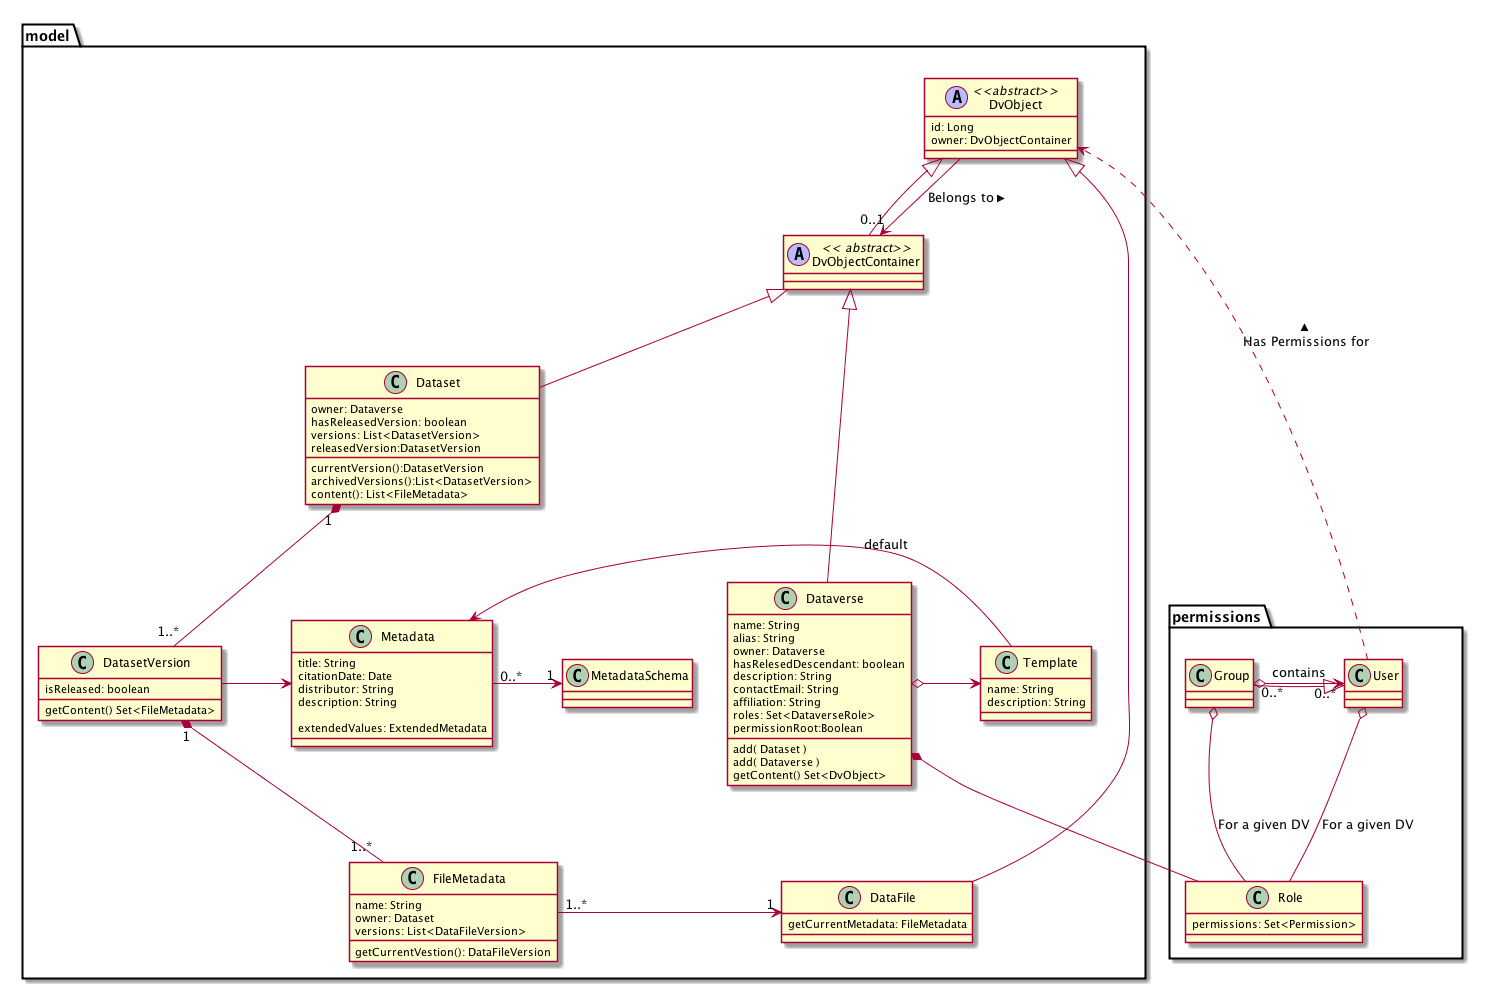
\includegraphics[width=\textwidth]{images/dataverse-model}
    \end{centering}
    \caption[The Dataverse class model]{The Dataverse class model\footnotemark[\getrefnumber{architecture}]}
    \label{fig:dataverse-model}
\end{figure}

In the heart of Dataverse is the division of content into Dataverses. The
closest analogue to a Dataverse is a normal folder in a typical file system -
Dataverses can contain other Dataverses, but in the place of files Dataverses
contain datasets. Datasets, in turn, contain the files that make up the
dataset. The Dataverse split of the system also allows for fine grained access
control, since Dataverses can be shared with no one, with single users or user
groups.

Users can use the Dataverse
with either the web user interface or the API offered by Dataverse. The
dataflow and interplay of the different components of the Dataverse application\footnotemark[\getrefnumber{architecture}] is shown in Figure
\ref{fig:dataflow}.

\begin{figure}
    \begin{centering}
        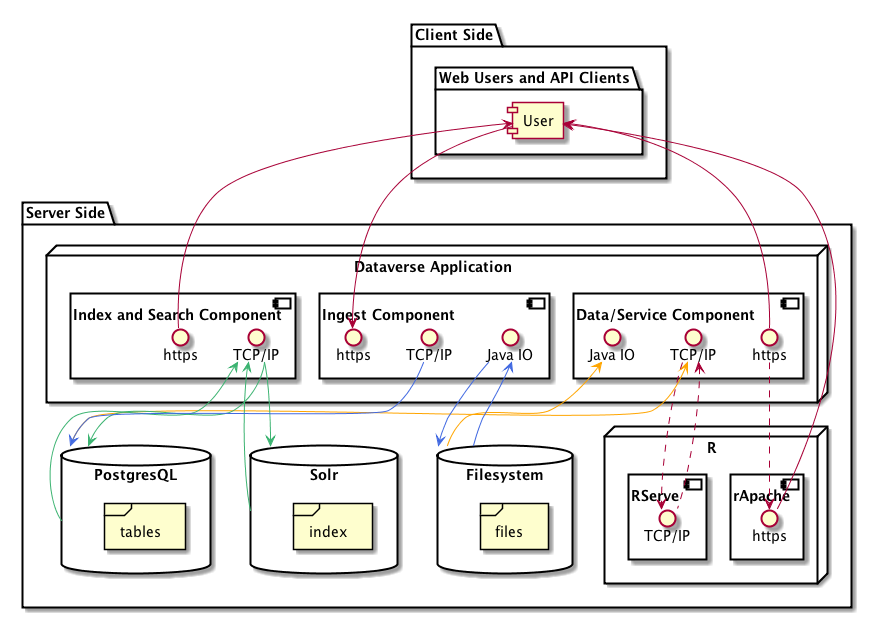
\includegraphics[width=\textwidth]{images/dataflow}
    \end{centering}
    \caption[The Dataverse application dataflow]{The Dataverse application dataflow\footnotemark[\getrefnumber{architecture}]}
    \label{fig:dataflow}
\end{figure}

The Dataverse Java application encompasses the Client Side and Dataverse
Application in Figure \ref{fig:dataflow}. Ingest refers to uploading datasets
to the system and the Index and Search and Data/Service components serve the
user the desired content, be it search results or data to be downloaded. The
rApache component handles the data visualization and runs the TwoRavens tool,
and RServe is used for the statistical computation when the user requests that.

Two versions of the Dataverse system were installed - one from source
code\footnote{\url{https://github.com/quarian/dataverse}} and one from the
installation bundle provided by the developers of
Dataverse\footnote{\url{https://github.com/IQSS/dataverse/releases/tag/v4.2}}.
The installations were run in the CSC cPouta
environment\footnote{\url{https://research.csc.fi/cpouta}}, which is an
OpenStack instance\footnote{\url{https://www.openstack.org/}}. The source code
installation is referenced from now as the development installation. It
was used to get a feel of the code and the system quality and the access
to the source makes debugging weird situations easier.
The installation from the installation bundle is referred to as the production
installation. The installation bundle should provide a more stable system than the branch of development
code that was forked for the development installation. Figure
\ref{fig:cpouta} shows the different installations in the cPouta environment.

\begin{figure}[t]
    \centering
    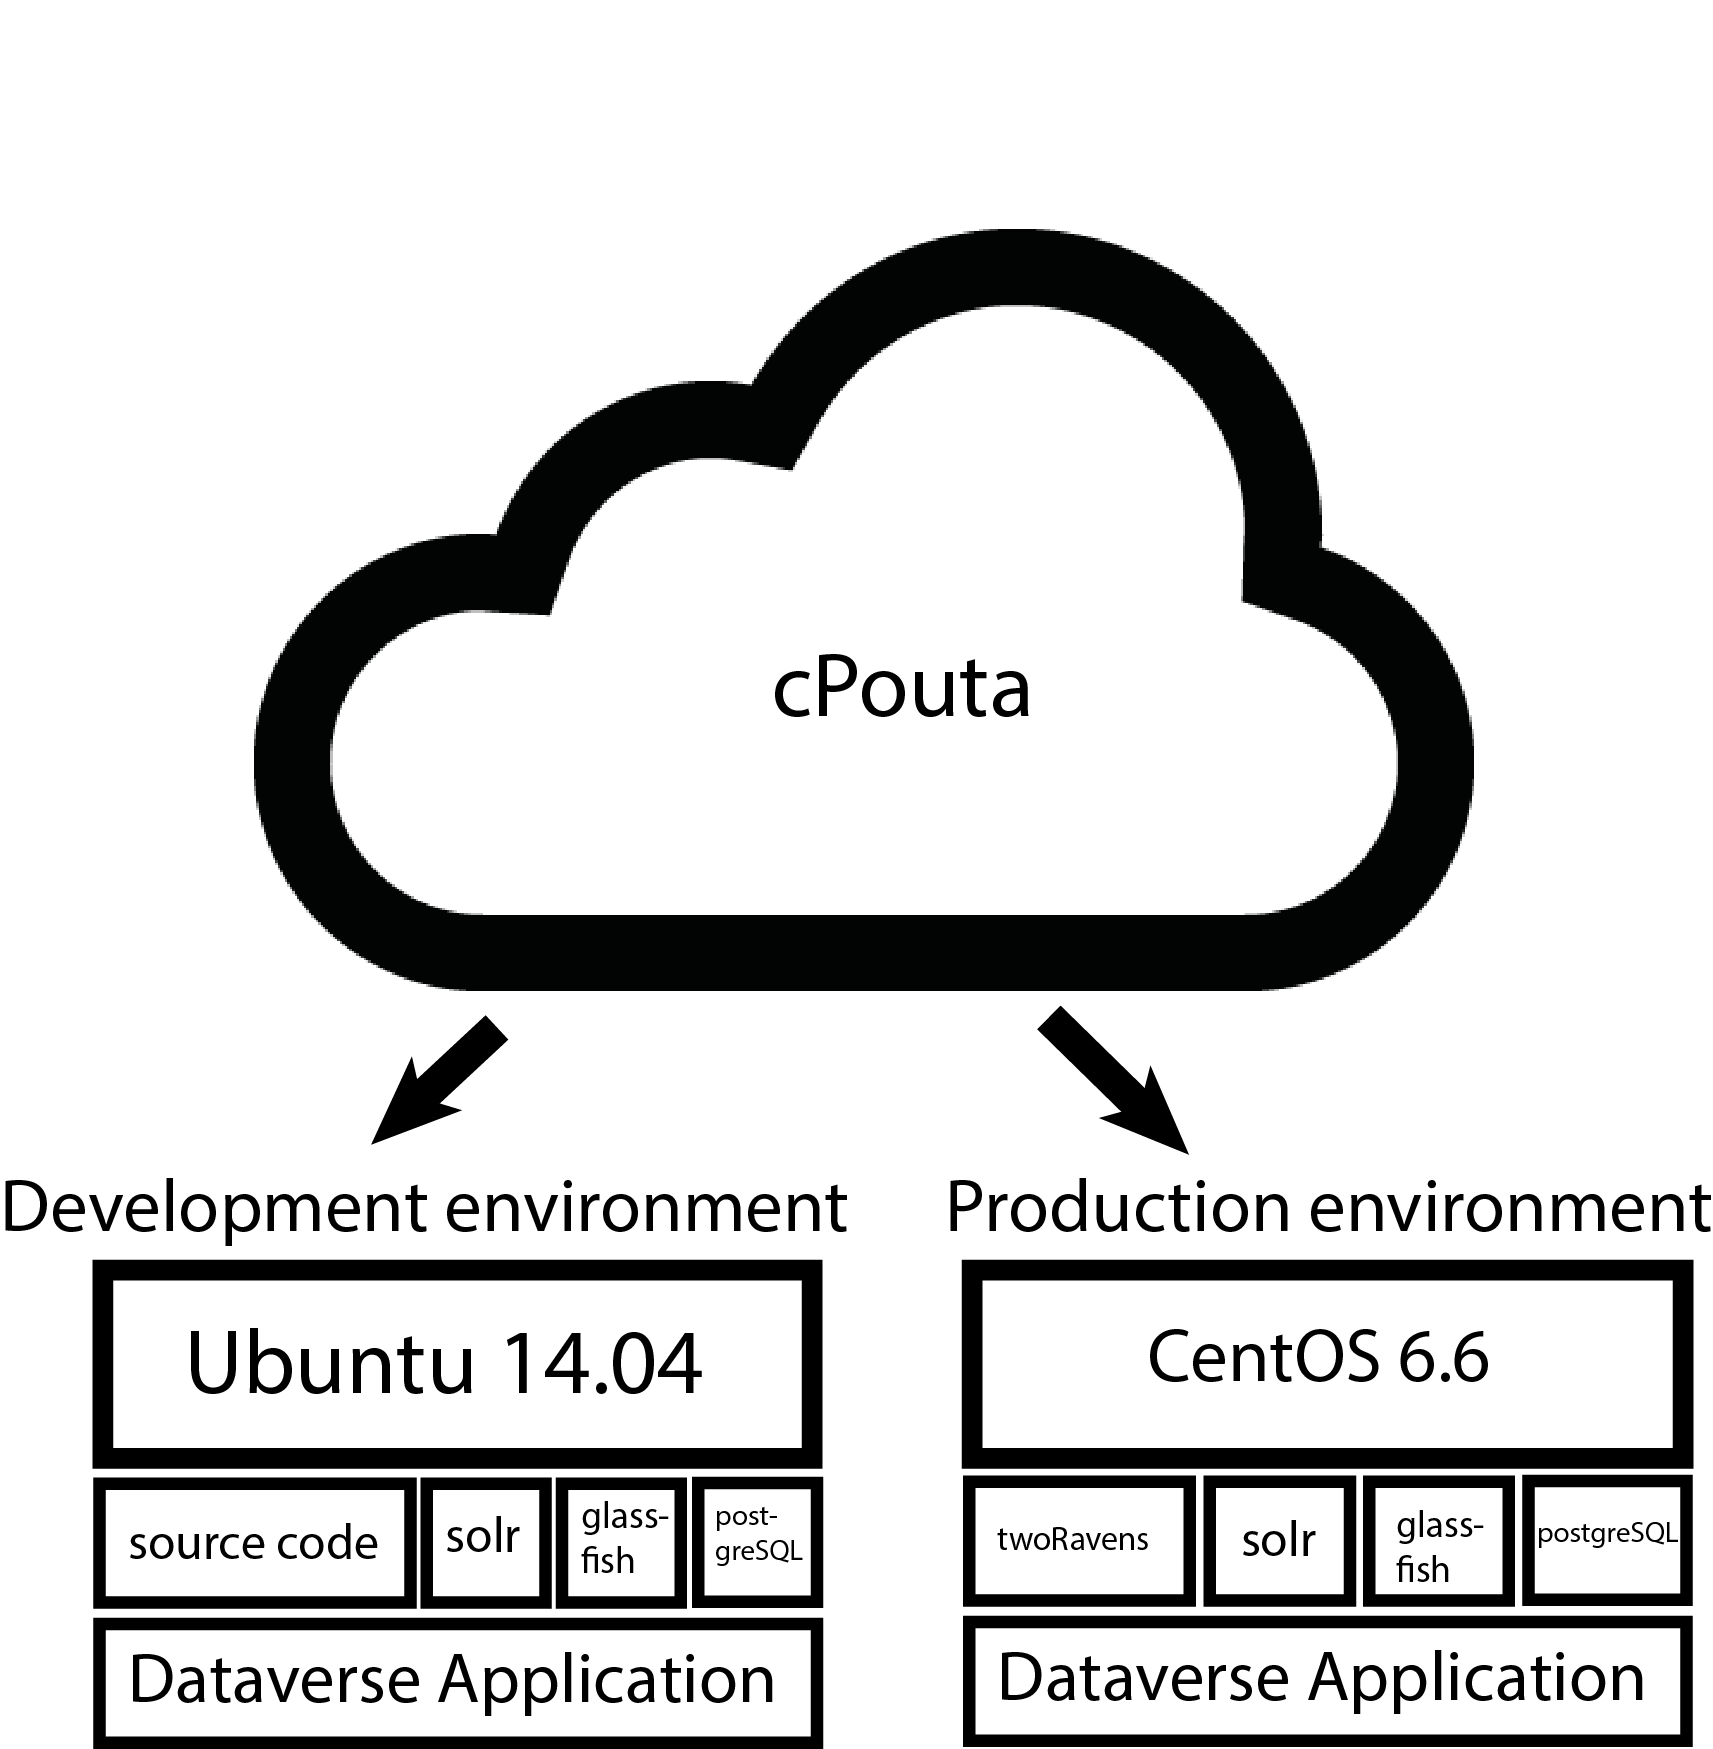
\includegraphics[width=0.7\textwidth]{images/cpouta2}
    \caption{The different installations in the cPouta environment}
    \label{fig:cpouta}
\end{figure}

The development installation is installed on top of Ubuntu 14.04 and it
works, even though the installation instructions propose the use of Red Hat
based systems. The TwoRavens application is omitted from the development
installation, since the data visualization is not the core functionality of
the research data repository software. The production installation is done
on CentOS 6.6, which is a derivative of Red Hat Linux. The installation was
first tried on CentOS 7.0, but the differences between CentOS 6.x and 7.x made
it so that the installation would not work - CentOS 6.6 was settled to be the
final environment of the development installation.

As for the information security of the prototype solution, the development
installation is not set up with any firewall rules or other security, since
its purpose is to get a feel of the system. For the production installation
firewall rules are set using the security groups functions of OpenStack.
Inbound TCP/IP traffic was only allowed to port 8080, which Glassfish was
listening to.
When it comes to research data, security is important, and since the
technologies such as Glassfish and postgreSQL are well known software and
their default passwords and ports are well known setting up firewalls and
changing those passwords is imperative. Additionally, with Dataverse,
firewalling the port that Apache Solr uses is important, since it circumvents
the user credentials and it could be used to retrieve any indexed information
in the system.

To replicate the test systems follow the installation
instructions\footnote{\url{http://guides.dataverse.org/en/latest/installation/}}
and the description here.

\section{System test setup}
\label{sec:system_testing}

In order to extract value from the prototype Dataverse it needed to be tested
with actual users. Of all the stakeholders groups presented in Section \ref{sec:users}
the research scientists is the most important one, since without them there is
no research data and without them using the research data repository there is
no public research data. Section \ref{chapter:positioning} summarizes learnings
from the other stakeholder groups. Section \ref{chapter:positioning} also contains results from
surveys conducted on research data management and sharing to provide context
also from the point of view of researchers.

To test this system we worked together with the Complex Networks
Group\footnote{\url{http://becs.aalto.fi/en/research/complex\_networks/}} and the
Speech Group\footnote{\url{http://research.ics.aalto.fi/speech/}} of Aalto
University. Two kinds of tests were designed and implemented. The first test was a contextual
interview - which means an interview and observation conducted in the user's normal working
environment. The contextual interviews were conducted both with
the development installation of the Dataverse as a tool for discussion and as
conversations and observations about the current state of research data management and the
current working practices. The second test was conducted with two lead users
and the production Dataverse installation. The users were asked to input their
datasets to the Dataverse and fill in the appropriate metadata.

The contextual interviews focused on the current methods of research data
management and sharing. The users were asked to describe their practices and
how they had come across to them (taught by the university, learned on their
own or some other methods). When applicable, the users were asked to show
their current setups for research data management and sharing. When the
development Dataverse was used the users were asked to upload a test dataset
to the Dataverse and walk the interviewer through the thought process. In
addition the interviewees were asked to use the actual Harvard
Dataverse\footnote{\url{https://dataverse.harvard.edu/}} to find datasets
relevant to their field of study and talk through the process. All these
interactions were also observed to find out usability and other issues that
might arise during the exchanges. In total 10 members of the Complex
Networks group were involved in the contextual interviews.

The lead users were granted access to the development Dataverse and were
briefly instructed to the different functionalities of Dataverse. The
instructions were left vague in order to make them read the relevant user
guides and provide feedback on how easy the system was to use after only very
brief instructions. After roughly a month's time the lead users were debriefed
and interviewed about their experiences with the Dataverse system.

The goal of these tests was to understand the current status of research data
management and publishing, how a research data publication system would fit
this status and how well does the research data publication system fill its
designated role. The usability of the system is also a point of interest.

In addition the installation and maintenance of the prototype installations
would give insight on how the system would be to maintain and how it would work
from a technical point of view.

\section{Outcomes of the prototype and the tests}
\label{sec:prototype_outcomes}

The contextual interviews and lead user tests yielded results on technical matters,
user interface and experience matters and on the current status of the research
data management and publishing.

The results of the tests showed that the technical implementations for research
data sharing fill their role. In the contextual interviews it was clear that
the manual uploading and searching worked fine - the users were able to pick up
the process of searching and uploading datasets quickly. The upload process is form
based, shown in Figure \ref{fig:upload} which is similar to many
form based upload pages you can find online. Files for datasets can be dragged and
dropped to the user interface or the file browser of the computer can be used. The users
were able to find the suitable method for them from the two options. But even
though the upload process is mechanically easy, the upload form contained a part
where the user was supposed to insert keywords of the dataset being uploaded.
The keywords come with the concept of vocabulary that was not known to the
users. The point of confusion is shown in Figure \ref{fig:vocabulary}. In this context vocabulary
refers to a set of words that have been agreed upon within a field of science
in order to standardize communication within the field.

\begin{figure}
    \begin{centering}
        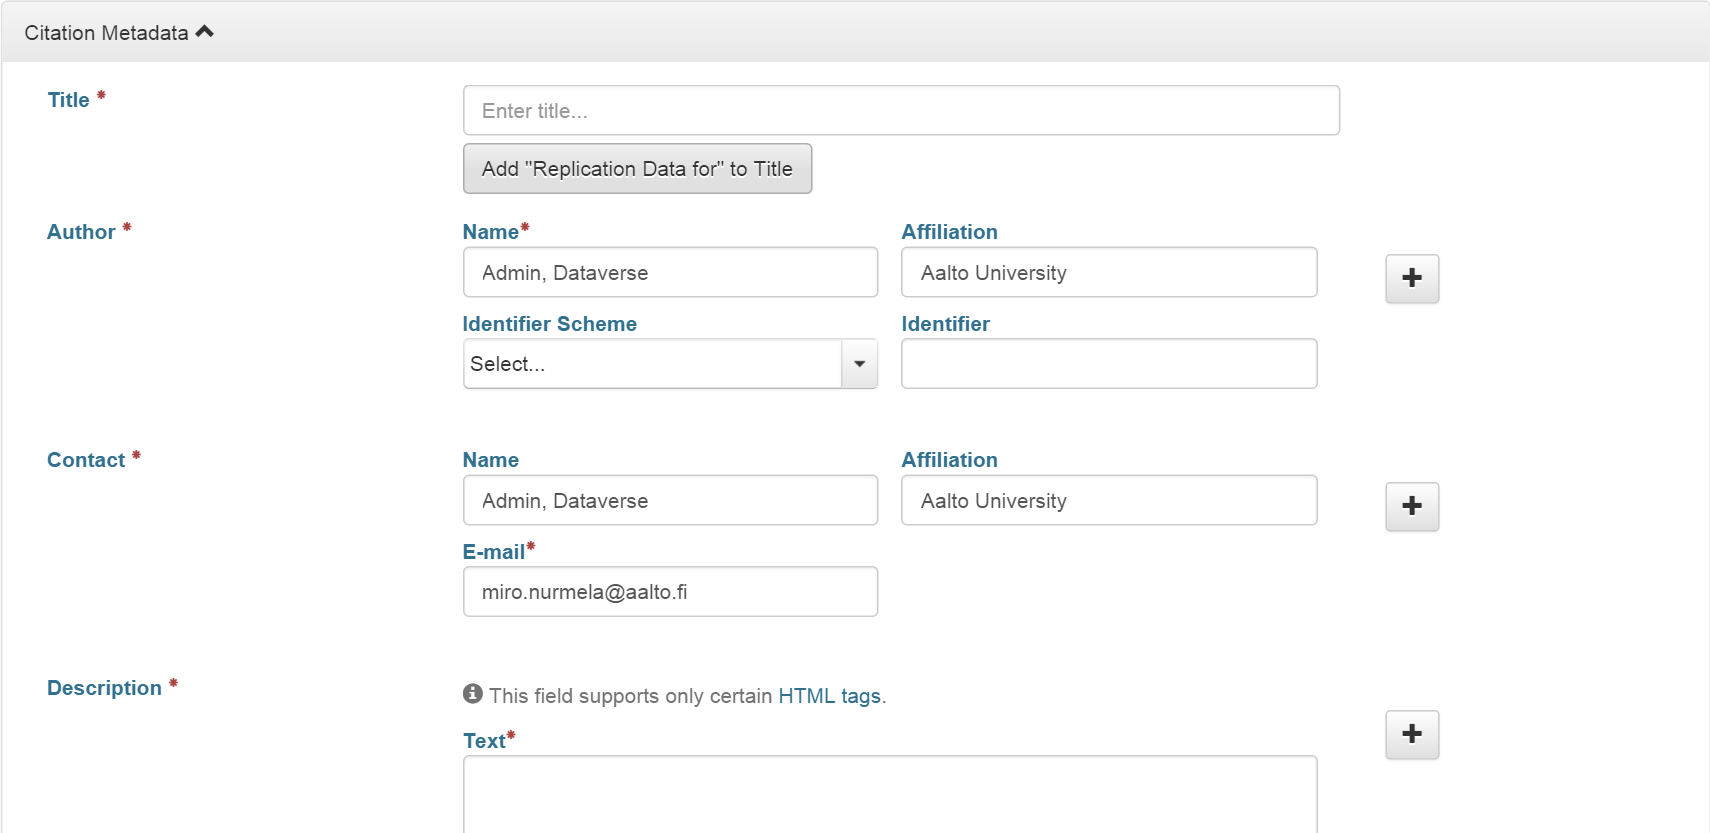
\includegraphics[width=\textwidth]{images/upload}
    \end{centering}
    \caption{A screen capture of the dataset upload form}
    \label{fig:upload}
\end{figure}

\begin{figure}
    \begin{centering}
        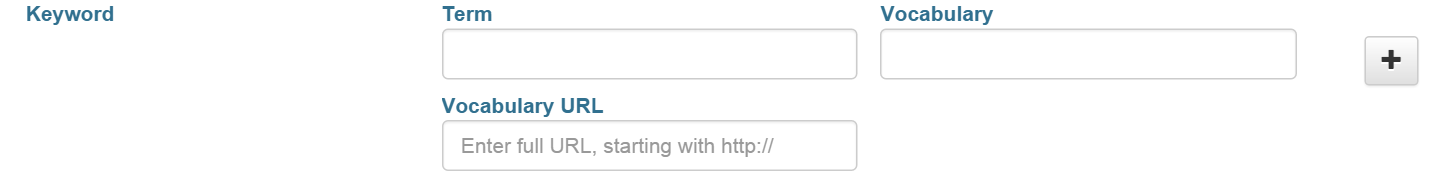
\includegraphics[width=\textwidth]{images/vocabulary}
    \end{centering}
    \caption{A screen capture of the confusion inducing vocabulary in the upload form}
    \label{fig:vocabulary}
\end{figure}

What is lacking of the upload process was the extended metadata that would be
important for the reuse of the data. The upload form contains the basic
metadata that is required to make the dataset searchable. Additional metadata,
such as details about the process of gathering the data, needs to be filled in
after the initial upload. The upload form contains a reminder, pictured in
Figure \ref{fig:hint}, to go add the metadata later. This approach has pros and
cons, since it makes the upload process easier but makes the metadata likely
lacking. Most users did not notice the hint to go add the metadata later and
those who did notice it did not know where the metadata addition would be done.

\begin{figure}
    \begin{centering}
        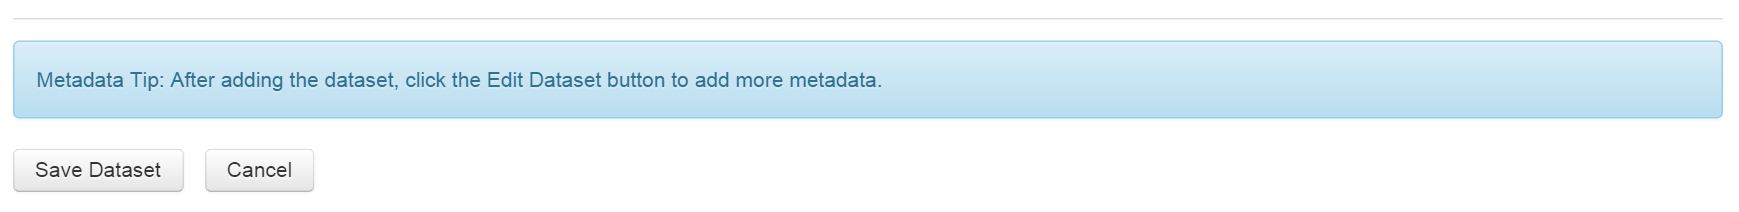
\includegraphics[width=\textwidth]{images/hint}
    \end{centering}
    \caption{A screen capture of the metadata reminder}
    \label{fig:hint}
\end{figure}

The search functionality is placed front and center in the user interface of
the Dataverse main page, as shown in Figure \ref{fig:search_main_page}. Users
easily locate the search bar and are able to start searching for relevant
datasets. The search results leave users lacking, however. This is not entirely
the fault of the search system, since the users found the names and short
descriptions of the datasets poor at describing the datasets which made
finding relevant datasets hard. Using the advanced search, which all the users
did not find, helps narrow down the options. The options in the
advanced search were noted to miss details. Details the users were missing
were dataset size and metadata related to their field. It was noted that
the system would work very well if you knew what you are looking for, for example
a scenario where your fellow researcher would have shared the identifier of
the dataset.

\begin{figure}
    \begin{centering}
        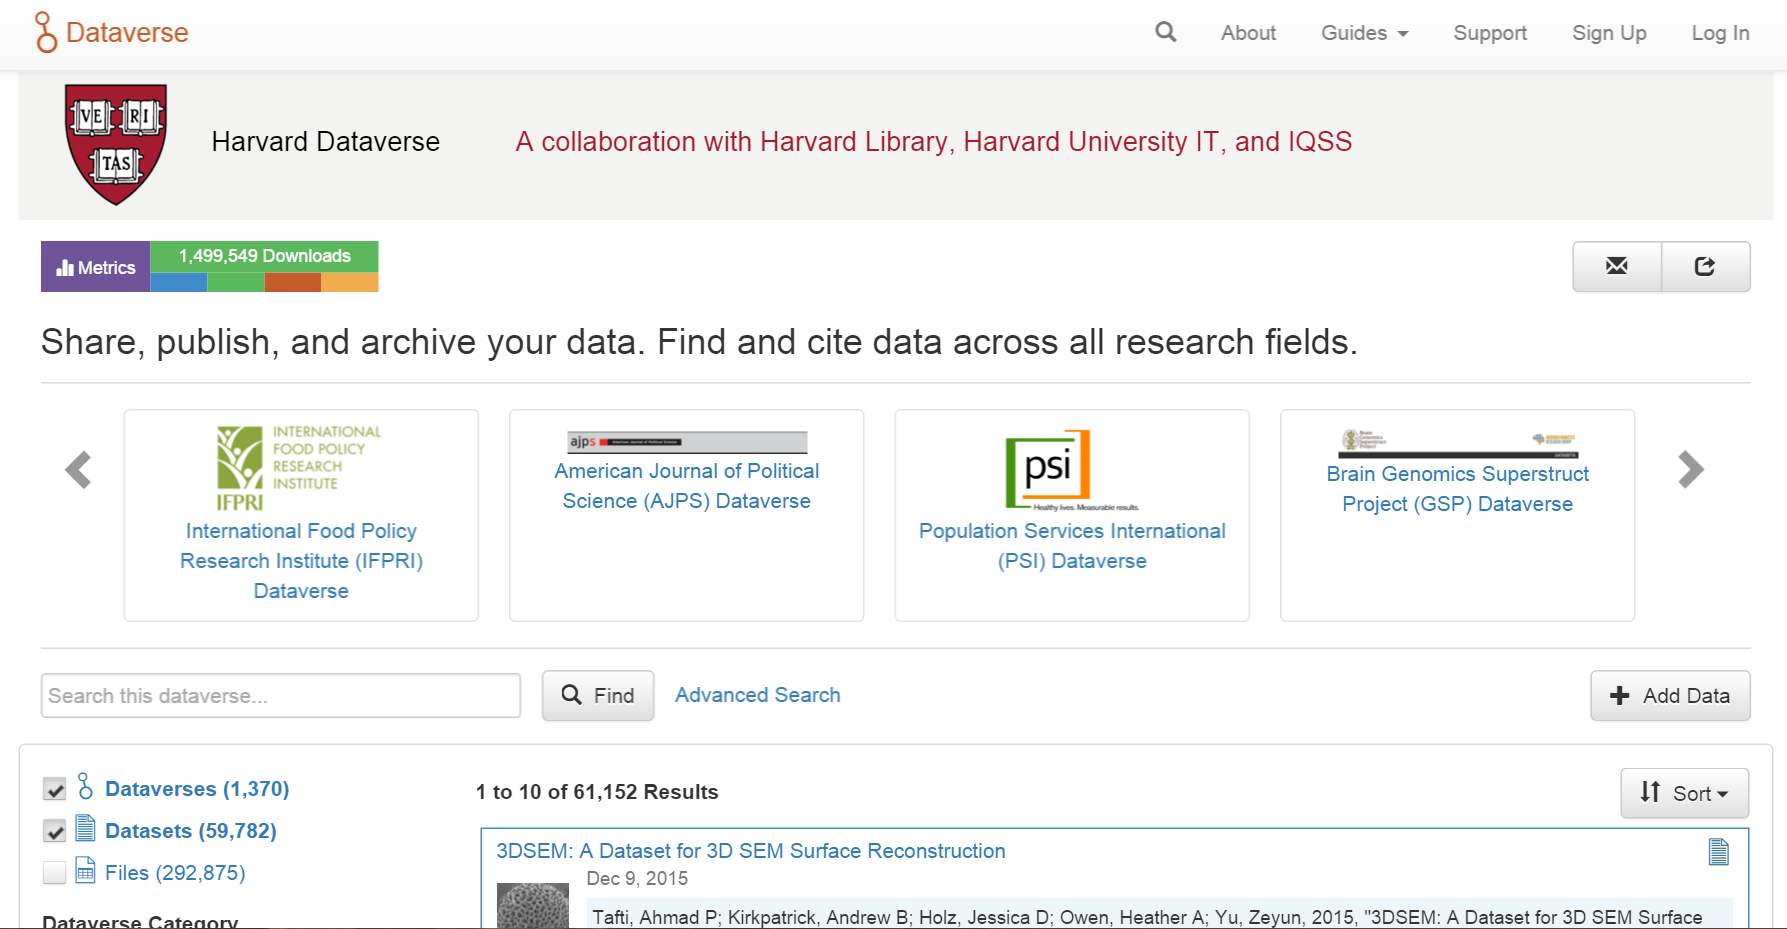
\includegraphics[width=\textwidth]{images/search_main_page}
    \end{centering}
    \caption{A screen capture of the Harvard Dataverse main page}
    \label{fig:search_main_page}
\end{figure}

The order in which the results are displayed is also unclear to the users.
The search results page offers the chance to sort the results, but that option
was missed by all users during the tests. The default setting is to sort the results by
relevance, but it is unclear to what relevance refers to in this context, since
the default search searches all searchable fields in datasets, Dataverses and files.
The fact that Dataverses, datasets and files are by default mixed in the search
results also does not help in finding relevant datasets. There is the option to
filter the files, datasets or Dataverses out of the search results, but the
option was fairly commonly missed by the users. It might be due to the novelty
of the terminology (Dataverse, especially, is a novel concept for the users).
An example of serch results is shown in  Figure \ref{fig:search_results}.

\begin{figure}
    \begin{centering}
        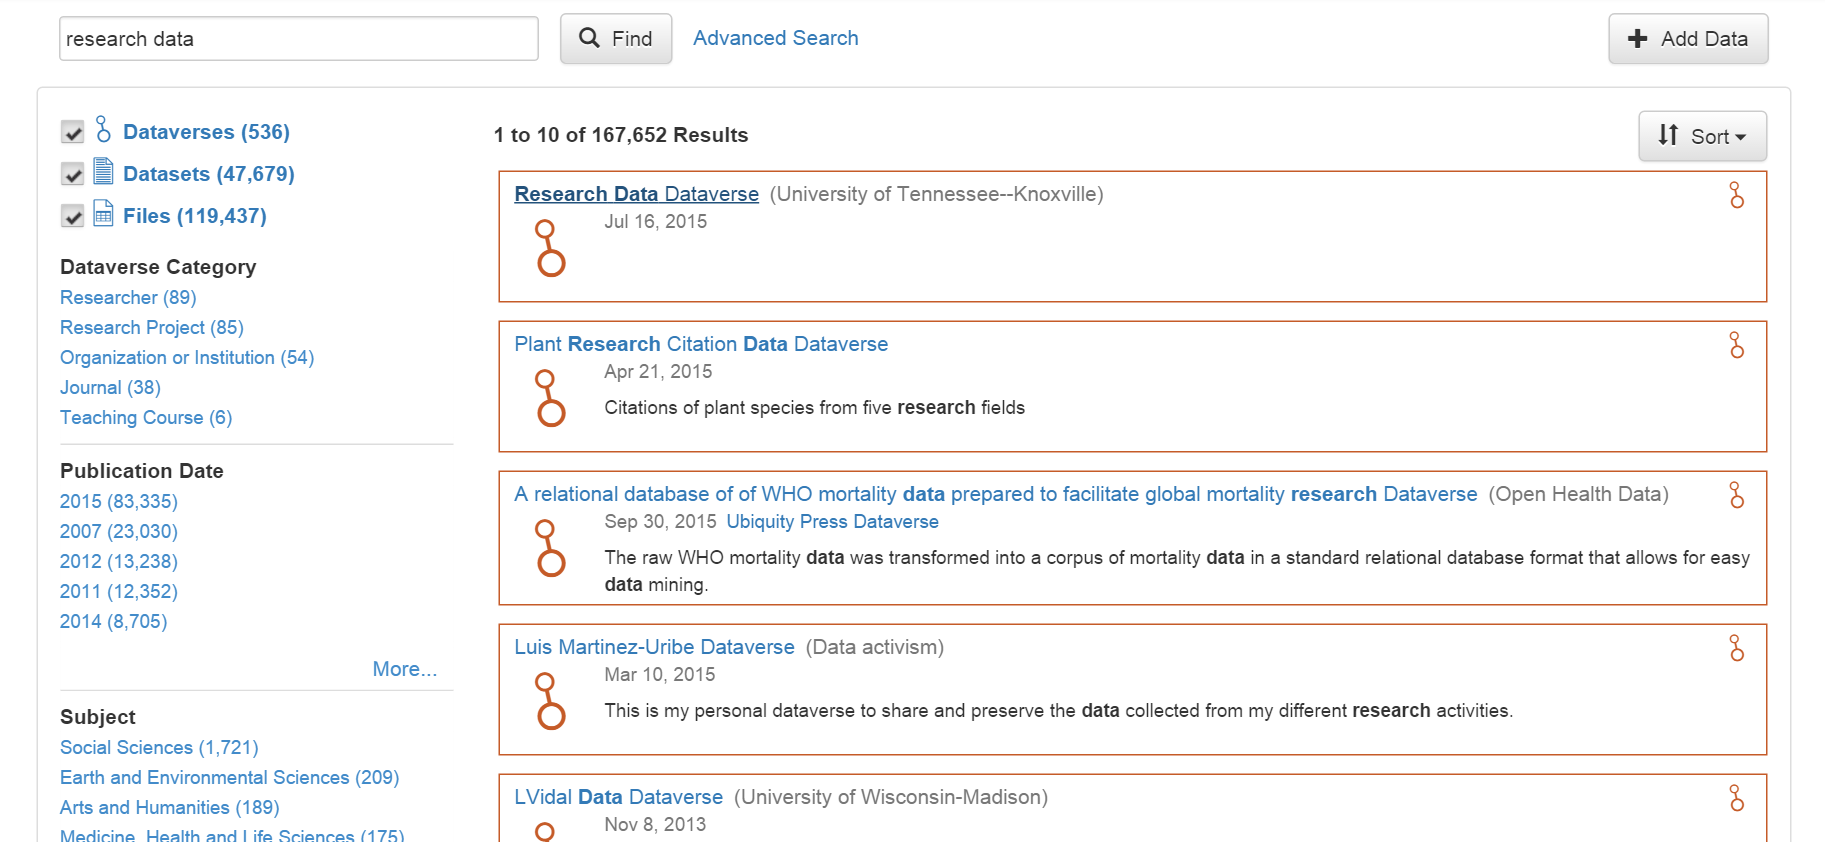
\includegraphics[width=\textwidth]{images/search_results}
    \end{centering}
    \caption{A screen capture of an example search results page}
    \label{fig:search_results}
\end{figure}

Dataverse implements helpful hover texts on the terms, as shown in Figure
\ref{fig:hovertext}. This feature went unnoticed by all users at first, but
most of them would find the feature by accident and find it helpful. It would
help if the helpful hover text would be indicated, for example, by a question
mark symbol next to the item to be explained.

\begin{figure}
    \begin{centering}
        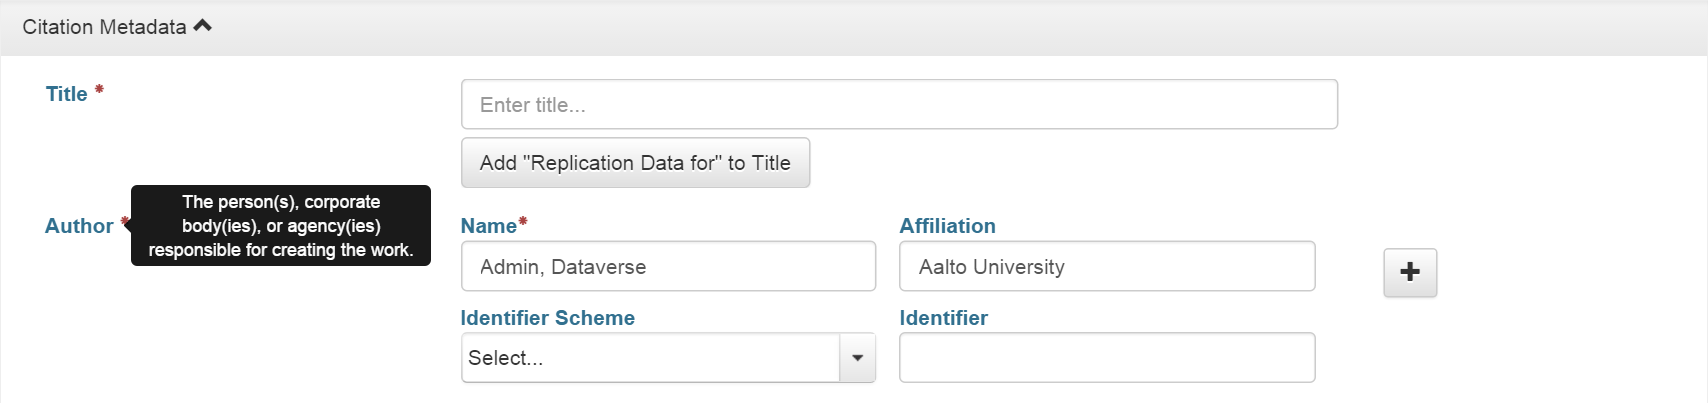
\includegraphics[width=\textwidth]{images/hovertext}
    \end{centering}
    \caption{A screen capture of the hover texts implemented in Dataverse}
    \label{fig:hovertext}
\end{figure}

What was common in both the contextual interviews and the lead user tests was
that the concept of publishing research data is novel for all the users. None
of them had published their research data online and few had used datasets from others,
but in those cases the datasets were always acquired by request and then
delivered using existing systems, such as Google Drive or email. When 
questioned on if they could make their research data public, for example with a tool
like Dataverse, many expressed that their research data had some privacy
concerns or other limitations to sharing or that it would take a considerable
amount of time to apply relevant metadata to make the datasets presentable.
Source code from some projects had been published in GitHub.

The contextual interviews and the lead user tests also shed light on the
current ways of managing research data. Network drives were used by the
users and their research groups to share all the data within the group, but
the there were no clear guidelines on how to describe dataset metadata or how
to organize the file structure on the network drives. This meant that it was
at times hard for the researchers to find relevant things from the drives and
for the new members of the groups to get acquainted with the system. It turned
out that currently research data management is not taught to the researchers,
but knowledge is gathered from peers and mistakes you make on your previous
projects.

The research data visualization, which came up as an interesting feature to
have in a research data publication platform during both the initial interviews
and the contextual interviews is implemented in Dataverse. The user feedback
on it, however, was that the visualization is very confusing and despite the
users being well versed in statistical methods could not understand what the
information displayed on the screen meant and how to get valuable information
out of it. Figure \ref{fig:tworavens} shows a view of the visualization tool.

\begin{figure}
    \begin{centering}
        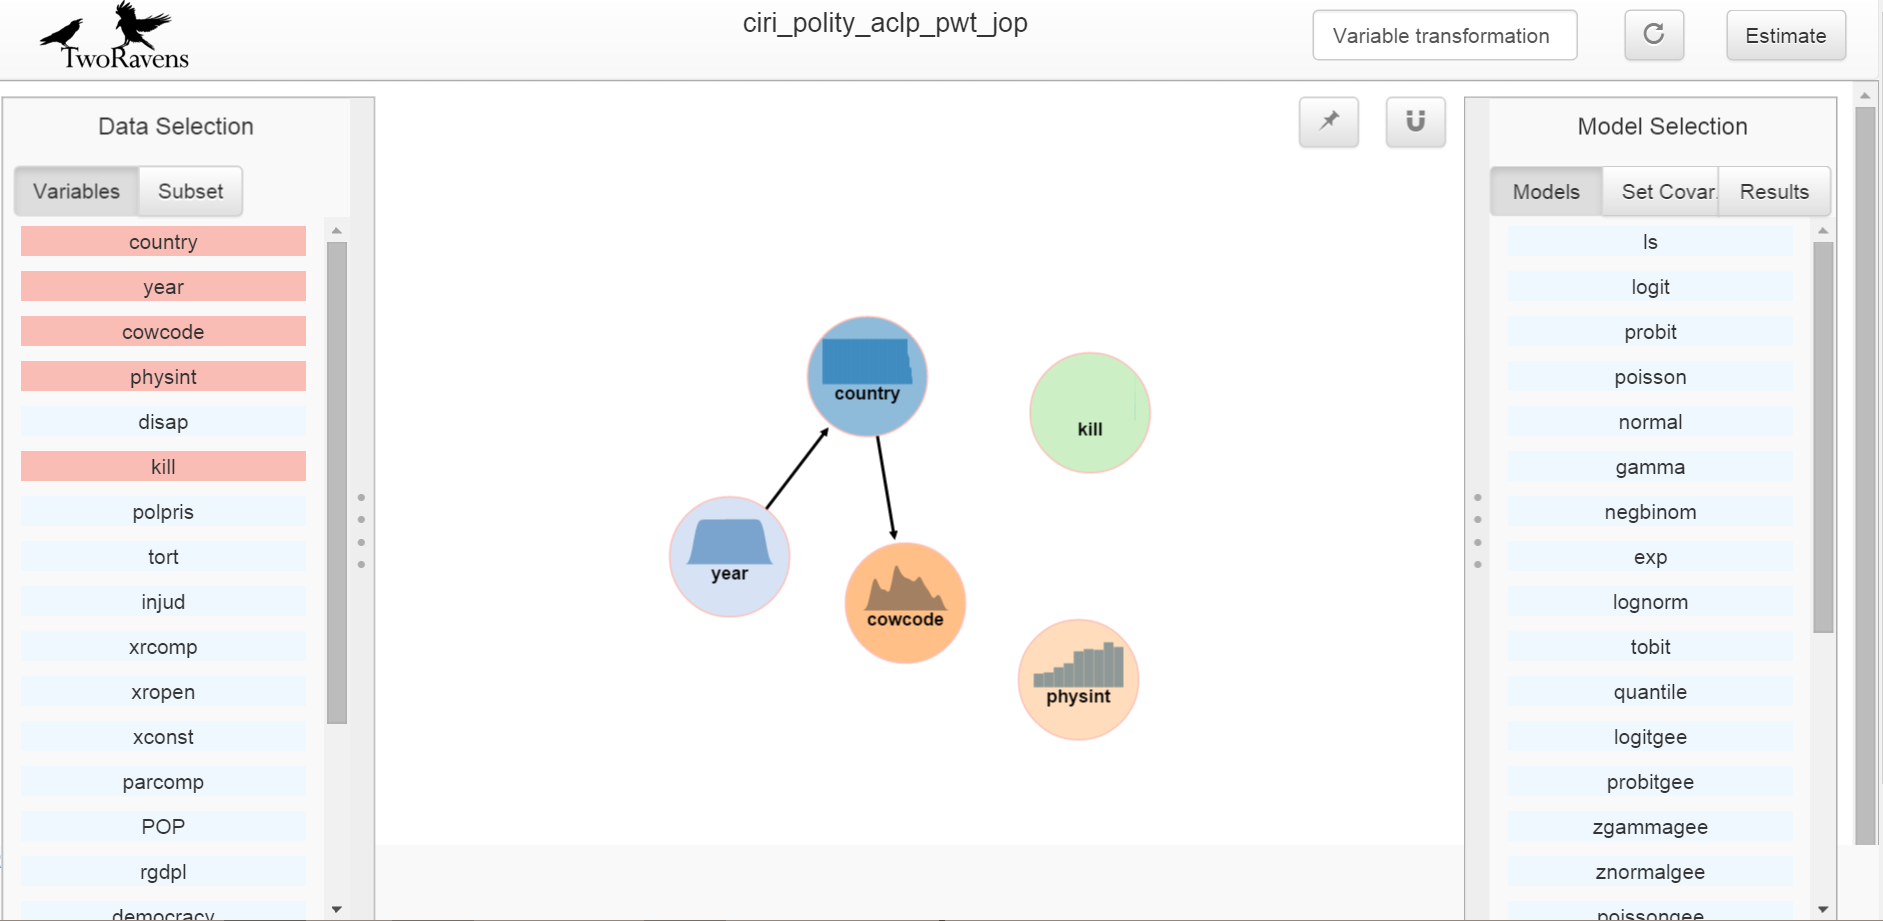
\includegraphics[width=\textwidth]{images/tworavens}
    \end{centering}
    \caption{A screen capture of Data visualization implemented in Dataverse}
    \label{fig:tworavens}
\end{figure}

The lead user tests mirrored the results from the contextual interviews when
it came down to the manual upload process of the datasets. Despite the lack of
previous knowledge on how to use the system or on how to publish research data
the lead users were able to learn the system and upload their datasets. After
working with the system for a longer time the need for computerized uploading
process became clear. For example, the user from the Sound Group had hundreds
of video files that could be uploaded to the publication system, but it would
not make sense to spend the time to do that manually. In addition some of that
data was being generated every day, so if that was to be published daily it
would require an automated system. The Dataverse offers a an API and a guide
for using it\footnote{\url{http://guides.dataverse.org/en/4.2/api/}}. The
user found that the guide with only example commands was
not enough to make the use of API easy.

After using the system for a longer time the users noted that the system could
help them access their datasets from outside the university's network. The
network drives and similar approaches in used nowadays limit the access to
the systems to the university network, which hinders both the ability of the
researchers to work on it from different computers as well as the ability to
share the information with collaborators from other places. There are, of
course, ways to access data within the university network with VPN or other
similar technologies, but that adds complexity to the process.

The longer period of use also brought up the fact that there is information in
how people store their data. For example, the folder structure of the network
drive might split files into subfolders by date of data collection. This serves
as implicit metadata, since there is no metadata file that tells that this
piece of data is from a certain date, but a human using the system would
understand it. Dataverse offers a chance to upload .zip file to the system
and this way preserving folder structures. In the case of
the Sound Group the video files are so large and there are so many of them
that uploading a huge file would make the reuse of that file very hard, not
to mention the uploading and downloading the file.

The installation and maintenance of the prototype Dataverse installation had
both flaws and good things to it. The basic installation following the
installation guide was easy, but adding in components like the TwoRavens or
Shibboleth authentication system was documented less clearly to the point that
it was not worth the effort to install the Shibboleth system for the prototype
solution. The TwoRavens installation process seemed to work, but the system
did not end up working in the prototype solution, so the TwoRavens was tested
with the actual Harvard Dataverse.

Codewise the Dataverse implementation is clean - it follows good object
oriented programming practices. Functionality is split into different
classes and the methods are short and well named. Dataverse has unit
tests implemented as well as a Jenkins
environment\footnote{\url{https://build.hmdc.harvard.edu:8443/}} for automated
integration tests. The test coverage is not very high - only
5\%\footnote{\url{https://coveralls.io/github/IQSS/dataverse}}.

User management with the Dataverse tools was easy. Dataverse offers a default
set of roles that cover the needs of research data publication process well.
Custom roles can also be made if the default ones are not enough.
Figure~\ref{fig:admin} shows the user management view of a single dataset. Permissions
can be changed for individual or groups, allowing the administrator of the
dataset to allow different parties to see the dataset before it is published.
Publishing will make it visible for all, but managing the permissions before
publishing the desired functionality of private publishing could be achieved.

\begin{figure}
    \begin{centering}
        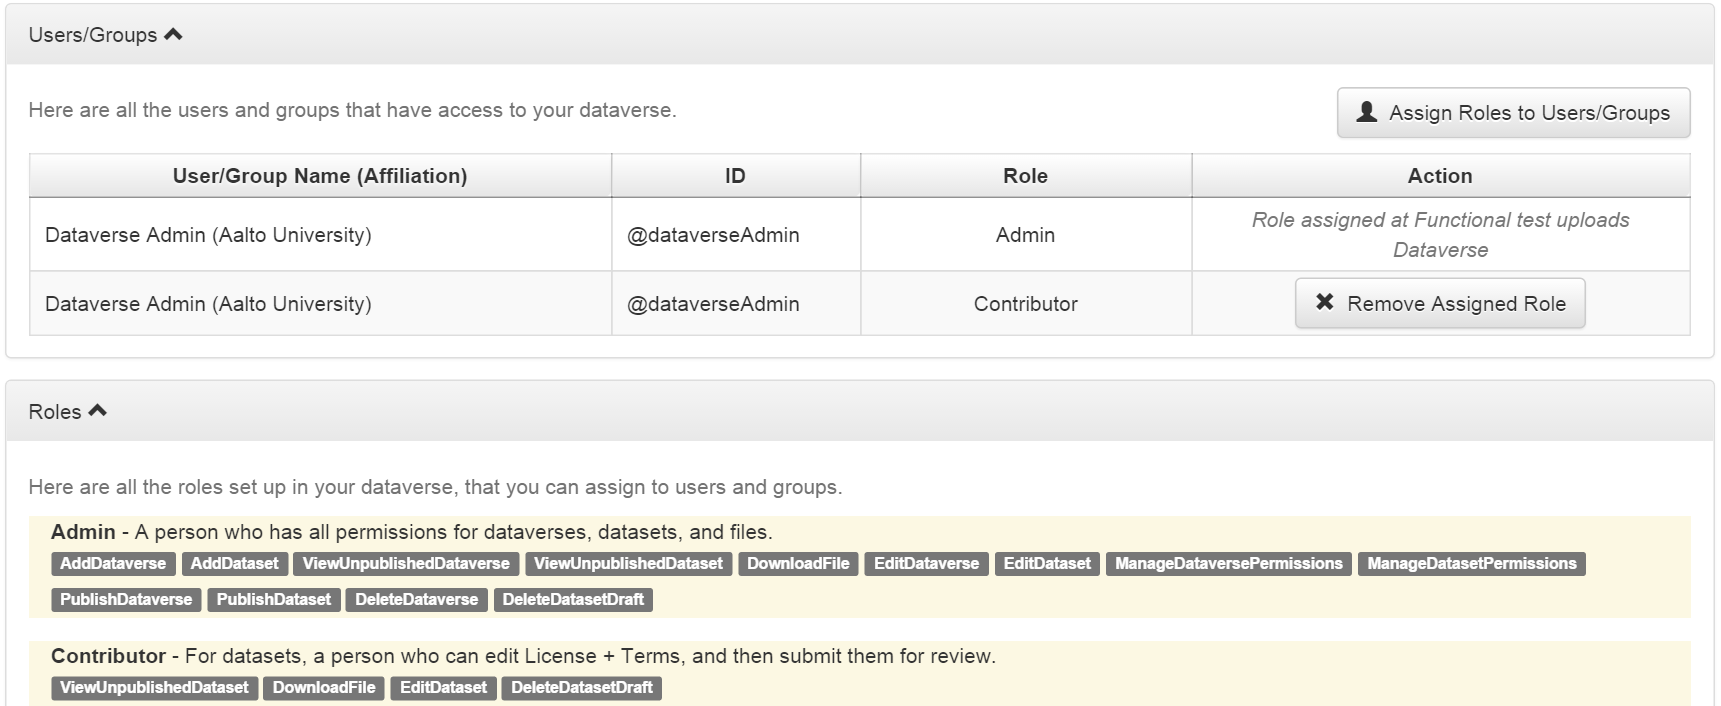
\includegraphics[width=\textwidth]{images/admin}
    \end{centering}
    \caption{A screen capture of the dataset user management view}
    \label{fig:admin}
\end{figure}

During the test on the development installation we came across an interesting
situation when the partition where the database of the Dataverse became too
full and no new datasets could be uploaded to the system. This did not crash
the system - the Dataverse could still be accessed and datasets be downloaded,
but new datasets could not be uploaded. Moving the database to a new partition
did not alone solve the problem since the failed dataset uploads had left
partial files to the Dataverse partition that prevented the Dataverse from
caching the new uploads. Once the fragmented remains of the failed uploads
were removed the and Dataverse had disk space to cache new datasets the system
started working again normally. It is good that the system was robust enough
to handle the insufficient space on the partition, but not cleaning up the
failed uploads caused frustration and the Dataverse documentation did not
help in resolving the issue.

Interesting note on Dataverse is that it gives DOIs to the published datasets.
This functionality is not documented, but digging into the code and the logs
from the system it turns out that that Dataverse uses the
EZID\footnote{\url{http://ezid.cdlib.org/}} service to supply DOIs for
datasets. What is strange is that when you set up your own Dataverse you
can just publish data and the DOIs will be given for you. This is strange
because registering DOIs is not free and it is hard to imagine that Harvard
would want to pay for all the DOIs for all the users of Dataverse.

In summary, Dataverse serves as a functional system to publishing research
data. The software is of good quality but the documentation and instructions
related to setting up the system could be better and the test coverage could be
improved. The mechanical processes of
uploading and searching datasets from the system work, but both of them could
be made more intuitive. Computerized upload of datasets is a must have feature
when dealing with datasets that contain a large amount of files. In addition to
taking care of these technical matters, training for research data management
and integration of research data publishing to the workflow of scientists is
required.

\iffalse
\begin{itemize}
    \item The manual uploading process is just fine
    \item It is a must that there is an API - for example, thousands of video
          files will not be uploaded manually
    \item It is important that the server can cache large files as a part of
          the upload process
    \item Search functionality
        \begin{itemize}
            \item Poorly described datasets
            \item Not intuitive to find data from within all the search results
            \item Dataset size is no available as a search filtering parameter
            \item The vocabulary in advanced search is foreign for the users
            \item The search results are not well organized
        \end{itemize}
    \item Access controls are important and function quite well
    \item Peer to peer teaching would be good
    \item How data is stored (folder structures and such) contains information
          and that should be captured by the system
    \item Accessing data from outside work computers would be nice
    \item More to come here, have to dig up my notes
\end{itemize}
\fi

 
\startchapright\chapter{Discussion}
\label{chapter:discussion}

\section{Methods}

In this thesis we examined the challenges around research data management,
sharing and publishing. The methods we used were literature reviews,
interviews, surveys, tehcnical benchmarks and user tests in the form of contextual
interviews and lead user tests.

Literature reviews on the subject revealed that while the open access way of
publishing research papers has been studied, the scientific contribution to
the problem of open acceess research data has been tackled ba a small number
of researchers. Statistical studies of open access benefits with research
papers promise good results for publishing open access style, but the
methodology and sample size quality varies. The metrics and numbers about
research data sharing and management are all different within the research
papers published, making it harder to interpret results from them. This is to
be expected, since research data publication and sharing is a relatively new
phenomenon. A challenge for the future would be to rigoriously quantify the
benefits of research data publication and sharing. Many of the research papers
in the field are also quite new, so it will take time to find out which ones
of them provide to be the most valuable.

Interviews were used to find out the current situation of research data
management and sharing in Finland. The interviewees represented many groups
of stakeholders, but it is possible that the people chosen for the interviews
were not the best representatives of their group. Legal issues were also
brought up quite a few times during this thesis and it would have been
beneficial to interview a legal expert as well. The interviews were conducted
in places chosen by the interviewees to make the interview process easier
for them. One possible failure case with the interviews was that they were
conducted alone, but this was taken into account by recording interviews.

The surveys were not designed for the use of this thesis, instead they were used
to find out the research data management needs of Aalto for planning the
future of services offered by Aalto. However, the questions asked in the
surveys were very relevant for this thesis as well which led to the decision
to use them as is instead of doing overlapping work. The general caveats of
surveys, such as the shallowness of information and the chance of
misinterpretation, apply of course. To minimize the the risk of misinformation
the results from the surveys were shown as is without too much interpretation.

Techincal benchmarking was done with existing solutions to varying degree.
The Dataverse solution was inspected thorougly, Zenodo and Hydra installations,
other publishing platforms were signed up for and tried that way and iRODS
was studied through the documentation and the code. There is a possibility
that the conclusions drawn from the thorough inspection of Dataverse don't
apply for the other solutions directly, but since the implementations are quite
similar the risk is likely low. We tried separating the lernings from the
systems from the system specific features, such as the look and feel of their
UIs. The cloud environment that was used as the basis of the prototype
Dataverse system would no the installation destination of the final system,
but it did not seem to generate problems for the testing.

The contextual interviews and lead user tests were chosen as a tool to learn
more about the research data publicatin systems to complement the technical
examination. It seemed that surveys would not provide adequate information on
a tool that did not exist yet and since Aalto is forming the data policy to
bring this sort of tools to the users it seemed that getting user feedback
in a controlled fashion from these tools would be beneficial. The sample size
of 12 users (10 for the contextual interviews and 2 for the lead user tests)
does not yeld statistically siginificant results, but the depth that the
examination was carried out with should provide value.

It was interesting that the interactions with the users of the system brought
up similar points that were raised in the literature. The lack of culture and
reasons for not sharing data were found out to be the same within these users.
Again, the sample size being so small this is nothing to write home about, but
it seems likely that the problems reported in literature around the world do
happen in Finland as well.

The goal of combining these methods was to gain a holistic view on the problem
and not only focus on the technological side.

The chosen methodologies were chosen also partially to accomodate the studies
of the writer of this thesis - I have studied user centered design as a my
minor during my masters' studies.

\section{Combining insights}

While the main focus of this thesis from the beginning was to find
appropriate techincal solutions for sharing research data it became clear
that sharing research data is not strictly a techincal problem. While there is
a lot of work to be done to make tools and systems to make the process of
sharing and publishing research data easy, a point solution to do just that
would fall flat. Firstly, research data publication and sharing is closely
tied to research data management during the research process. If research data
is not handled during the process with the goal of one day making it public,
the process of eventually making it public is very hard or impossible. And even
though it might be techically viable the time and effort it would take to
turn datasets that have not been properly documented and maintained during the
process might be prohibitive. Secondly, the culture for sharing research data
is not there yet. There is no knowledge about either research data management
or sharing. Additionally, there is no incentive to share research data, since
researchers' contribution is measured mainly in citation to research papers.

The problem of research data also involves people from different disciplines
in unprecedented ways. The roles of libraries, university software
infrastructure maintainers and the researchers themselves are undefined in
the new world of research data management, publication and sharing. And then
if you throw in the publishers and the peer review process that is in the
heart of the scientific publishing game it is clear that the roles of all
these actors need to be defined in the research data context.

Making research data accessible is likely to promote the quality of science.
To achieve this, better techical solutions need to be implemented and the
culture around research data needs to be taken into a more open direction.

\section{Future work}

In the previous section we discussed what would be need to make research data
more open. Future work around the subject should include both integrated
techincal solutions that make good research data management a part of the
daily life of researchers and thus making the publication of their data easy.
The change the culture more research on the benefits of open research data
is required, but there might be other ways as well.

Some fields of science, such as physics, psychology and genomics have been
more succesful than other in implementing open research data practices.
Research on how they managed that transition and how that could be applied
to other fields could find ways to bring open research data to other
fields as well.

It's also possible that the culture of research data could be changed with
appropriate sticks and carrots. If funding bodies would make it a priority
to demand public research data, there would likely be an urgency to provide
such solutions for researchers as soon as possible. On the other hand, maybe
citations to research data could be integrated to the h-index of researchers,
thus making the already used metric reward those who publish their datasets.
This reframing of the problem - instead of asking "how should we implement
such systems that help with research data?" we ask "how do we motivate people
to share their research data" - is a design paradigm that has been used
succesfully in other system level design problems \cite{dorst2015frame}.

The solutions for the technical and cultural problems might also be found
from analogous problems. For example, software development has benefited for
a long time from the open source community, where people contribute code for
the public domain without compensation. It's been studied that people do not
do this out of the kindness of their hearts, but instead with the goal of
turning their free work now into profit in the future
\cite{DBLP:conf/hicss/HarsO01}. The tools that are used to share software,
such as GitHub, could also provide a fresh look on how tools for research
data management and sharing could work.

\iffalse
In this chapter we'll discuss the findings, methods and such in a good
scientific manner.

At some point I want to discuss the analogue of software open source community
and how that works - how we should make people proud of making good, usable
datasets and sharing them.

\cite{DBLP:conf/hicss/HarsO01} is about the motivations behind working on open
source software - could be used for analogue for open data.

\cite{dorst2015frame} is the Kees Dorst book about reframing problems, which in
this case would be taking the technical problem of sharing reserch data, which
is not the actual problem, and reframing it as the problem on how to motivat
people to to share their data.
\fi


\startchapright\chapter{Conclusions}
\label{chapter:conclusions}

This thesis has examined different technical solutions to managing, sharing and
publishing research data, focusing on sharing and publishing.
Table~\ref{table:solutions} shows the features of solutions presented and shows
how they differ in the context of research data publishing, whereas Table~\ref{table:management} shows the same solutions but in the context of research
data management during a research project. Table~\ref{table:legend_colors} shows the legend that is used in
Tables~\ref{table:solutions} and \ref{table:management}. Research data is referred
to as data in the tables for a more concise presentation.

\captionof{table}{The color coding of the summary Tables \ref{table:solutions} and \ref{table:management}}
\addtocounter{table}{-1}
\label{table:legend_colors}
    \begin{tabularx}{\textwidth}{| >{\raggedright}p{3cm} | X |}
    \hline
    \textbf{Color and Mark} & \textbf{Meaning} \\
    \hline
    \multicolumn{1}{|c|}{\cellcolor{green}++} & The feature is well implemented and could be considered a strong point
                          in the solution \\
    \hline
    \multicolumn{1}{|c|}{\cellcolor{yellow}+} & The feature is implemented in the solutions in some way - it might need
                          some work to get up and running or the other features of the solution can be used to
                          approximate the functionality \\
    \hline
    \multicolumn{1}{|c|}{\cellcolor{red}-}    & The feature is missing from the solution or can be found from the solution but according
                          to user feedback is too hard to use and is a clear weak point of the solution \\
    \hline
\end{tabularx}

In Tables \ref{table:solutions} and \ref{table:management} the IDA, Etsin, Avaa and PAS are a part of the
Finnish Open Science Initiative. Dataverse, Hydra, Zenodo, iRODS and CKAN are
open source solutions. EUDAT refers to the B2-offering\footnote{\url{http://eudat.eu/}},
of which the B2Share and B2Drop are considered to be a part of a research
data management and publication process. ACRIS is the Elsevier Pure instance
that is being trialed at Aalto University. GitHub is included in the
comparison since it is a widely adopted tool for publishing and collaborating
on software projects.

The features used in the columns in Table \ref{table:solutions} are explained
in Table \ref{table:solution_features}.

\pagebreak

\captionof{table}{The features being compared on Table \ref{table:solutions}}
\addtocounter{table}{-1}
\label{table:solution_features}
    \begin{tabularx}{\textwidth}{| >{\raggedright}p{3cm} | X |}
    \hline
    \textbf{Feature} & \textbf{Explanation} \\
    \hline
    \rowcolor{Gray}
    Data Storage    & Data storage means that the solution offers the chance to
                      save the actual research data to the system and not just links
                      to the datasets, for example\\
    \hline
    Metadata Storage &  Metadata storage means that the system has a structured way
                        of storing metadata about datasets - this does not mean that
                        the system should contain actual research data, since some services
                        are built just as places to store metadata and links to datasets\\
    \hline
    \rowcolor{Gray}
    Open Access Data    & System that implements this feature allows the datasets to be searched
                          and downloaded by the general public without restrictions to the use
                          of the datasets\\
    \hline
    Restricted Data    & Whereas open access data is available for all the world to see, systems
                         that implement the restricted data feature allow for a more fine grained
                         user management allowing datasets to be shared with restricted groups
                         of users\\
    \hline
    \rowcolor{Gray}
    Long Term Archival    & Long term archival is archival for datasets that lasts for tens of years -
                            a lot longer than commodity hard drives last in active use (commodity
                            hard drives usually last from three to five years in active use)\\
    \hline
    Full Text Search    & Full text search refers to the ability to search the all the metadata
                          available in the system to find relevant datasets\\
    \hline
    \rowcolor{Gray}
    Dataset Versioning    & Dataset versioning means that the system allows for uploading newer versions
                           of the already uploaded datasets without deleting the old datasets, since
                           someone might use and refer to the old datasets\\
    \hline
    Identifier Scheme    & Identifier scheme tells which, if any, persistent identifier schemes the
                           solution implements\\
    \hline
\end{tabularx}

From the solutions presented in Table \ref{table:solutions} the systems that
are designed primarily for research data publishing (Avaa, Dataverse, Hydra,
Zenodo, and CKAN) have almost all the features specified. What some of
them are lacking is the ability to restrict access to the research data, which
is a requirement for some datasets that contain data that has some
confidentiality clauses. Avaa, for example, is a platform for nothing else than
completely open data making it an awkward choice for a university, for example.
None of these solutions implement long term archival,
which is an important feature going forward and a goal for future development.
These solutions are also remarkably similar, so any one of them could be used
to set up a research data publishing platform for a research institution.

The only solution for long term archival is PAS, which is in test phase as of
writing of this thesis. It ticks many boxes of the features, but it has to be
taken into account that the PAS system is only for long term archival and
can not be used for the normal publishing activity of research institutions.
It is also unclear at the moment how datasets for long term archival are
chosen, what kind of metadata long term archival requires and how the system
should integrate to existing and upcoming research data repositories.

The tools that have a lot of other functionality in addition to research data
publishing implement the features to a varying degree. iRODS, which is a tool
for managing data, is clearly not designed to be a data sharing platform for
research data. ACRIS has many other tasks as well, such as maintaining a the
publication profile of researchers and reporting publications. EUDAT's B2Share
offering offers a serviceable research data publication platform, but lacks the
ability to restrict access to the datasets in a fine grained manner. IDA is an iRODS based system, but
has some features for publishing datasets from the system. Biggest problem with
it is that it is perceived very hard to use by users.

Etsin is a metadata publication platform - it only contains metadata and links
to the actual location of the datasets. While this is valuable, separating the
research data from the metadata requires either integration between the storage
and metadata systems or more work from the users. This is also the reason why
Open Access Data is marked as a weakness of the system - no data, no open access.

The identifier scheme is also a point of interest. Citing datasets is something
that has not been widely adopted, which means that in order to help that
adoption a well known identifier scheme should be used. It is good that
a Finnish identifier scheme exists, but if datasets want international recognition
an internationally known identifier scheme should be used.

The technical solutions with a focus on research data publishing fill their
role adequately. The user tests show that there are user experience and
usability improvements that could be done - those are detailed in Section
\ref{sec:prototype_outcomes}. What the user tests also show is that training
related to the options when it comes to research data publishing is lacking.
If the culture and willingness to share research data is to be improved,
that would require a conscious effort from the university side.

\begin{sidewaystable}[h]
    \caption{Existing solutions in light of research data publishing}
    \label{table:solutions}
    \resizebox{\textwidth}{!}{
        \renewcommand{\arraystretch}{2.0}
        \begin{tabular}{| l | c | c | c | c | c | c | c | c | c |}
            \cline{3-10}\cline{1-1}
            \rowcolor{top-level-blue}
            \vspace{1 mm}
            \textbf{Tool} &\cellcolor{white}& \textbf{Data Storage} & \textbf{Metadata Storage} & \textbf{Open Access Data} & \textbf{Restricted Data} & \textbf{Long Term Archival} & \textbf{Full Text Search} & \textbf{Dataset Versioning} & \textbf{Identifier Scheme} \\
            \cline{3-10}\cline{1-1}
            \cellcolor{first-column-blue}IDA     && \cellcolor{green}++ & \cellcolor{yellow}+ & \cellcolor{yellow}+  & \cellcolor{yellow}+  & \cellcolor{red}-  &  \cellcolor{green}++ & \cellcolor{red}-  & \cellcolor{green}URN \\
            \cline{3-10}\cline{1-1}
            \cellcolor{first-column-blue}Etsin   && \cellcolor{red}-  & \cellcolor{green}++ & \cellcolor{red}-  & \cellcolor{red}-  & \cellcolor{red}-  &  \cellcolor{green}++ & \cellcolor{red}-  & \cellcolor{green}URN \\
            \cline{3-10}\cline{1-1}
            \cellcolor{first-column-blue}Avaa    && \cellcolor{green}++ & \cellcolor{green}++ & \cellcolor{green}++ & \cellcolor{red}-  & \cellcolor{red}-  &  \cellcolor{green}++ & \cellcolor{red}-  & \cellcolor{green}URN \\
            \cline{3-10}\cline{1-1}
            \cellcolor{first-column-blue}Dataverse && \cellcolor{green}++ & \cellcolor{green}++ & \cellcolor{green}++  & \cellcolor{green}++ & \cellcolor{red}-  &  \cellcolor{green}++ & \cellcolor{yellow}+  & \cellcolor{green}DOI/Handle \\
            \cline{3-10}\cline{1-1}
            \cellcolor{first-column-blue}Hydra    && \cellcolor{green}++ & \cellcolor{green}++ & \cellcolor{green}++ & \cellcolor{green}++ & \cellcolor{red}-  &  \cellcolor{green}++ & \cellcolor{yellow}+  & \cellcolor{green}DOI \\
            \cline{3-10}\cline{1-1}
            \cellcolor{first-column-blue}Zenodo   && \cellcolor{green}++ & \cellcolor{green}++ & \cellcolor{green}++ & \cellcolor{yellow}+  & \cellcolor{red}-  &  \cellcolor{green}++ & \cellcolor{yellow}+  & \cellcolor{green}DOI \\
            \cline{3-10}\cline{1-1}
            \cellcolor{first-column-blue}EUDAT    && \cellcolor{green}++ & \cellcolor{green}++ & \cellcolor{green}++ & \cellcolor{yellow}+  & \cellcolor{red}-  &  \cellcolor{green}++ & \cellcolor{yellow}+  & \cellcolor{green}Handle \\
            \cline{3-10}\cline{1-1}
            \cellcolor{first-column-blue}iRODS    && \cellcolor{green}++ & \cellcolor{yellow}+ & \cellcolor{red}-  & \cellcolor{red}-  & \cellcolor{red}-  &  \cellcolor{green}++ & \cellcolor{yellow}+  & \cellcolor{red}- \\
            \cline{3-10}\cline{1-1}
            \cellcolor{first-column-blue}CKAN     && \cellcolor{green}++ & \cellcolor{green}++ & \cellcolor{green}++ & \cellcolor{green}++ & \cellcolor{red}-  &  \cellcolor{green}++ & \cellcolor{yellow}+  & \cellcolor{yellow}+ \\
            \cline{3-10}\cline{1-1}
            \cellcolor{first-column-blue}ACRIS    && \cellcolor{red}-  & \cellcolor{yellow}+  & \cellcolor{yellow}+  & \cellcolor{yellow}+  & \cellcolor{red}-  &  \cellcolor{green}++ & \cellcolor{red}-  & \cellcolor{yellow}+ \\
            \cline{3-10}\cline{1-1}
            \cellcolor{first-column-blue}PAS      && \cellcolor{green}++ & \cellcolor{green}++ & \cellcolor{green}++ & \cellcolor{red}-  & \cellcolor{green}++ &  \cellcolor{green}++ & \cellcolor{red}-  & \cellcolor{green}URN \\
            \cline{3-10}\cline{1-1}
            \cellcolor{first-column-blue}GitHub   && \cellcolor{green}++ & \cellcolor{yellow}+  & \cellcolor{green}++ & \cellcolor{green}++ & \cellcolor{red}-  &  \cellcolor{green}++ & \cellcolor{green}++ & \cellcolor{green}DOI \\
            \cline{3-10}\cline{1-1}
        \end{tabular}
    }
\end{sidewaystable}

\clearpage

\iffalse
\begin{sidewaysfigure}
    \begin{centering}
        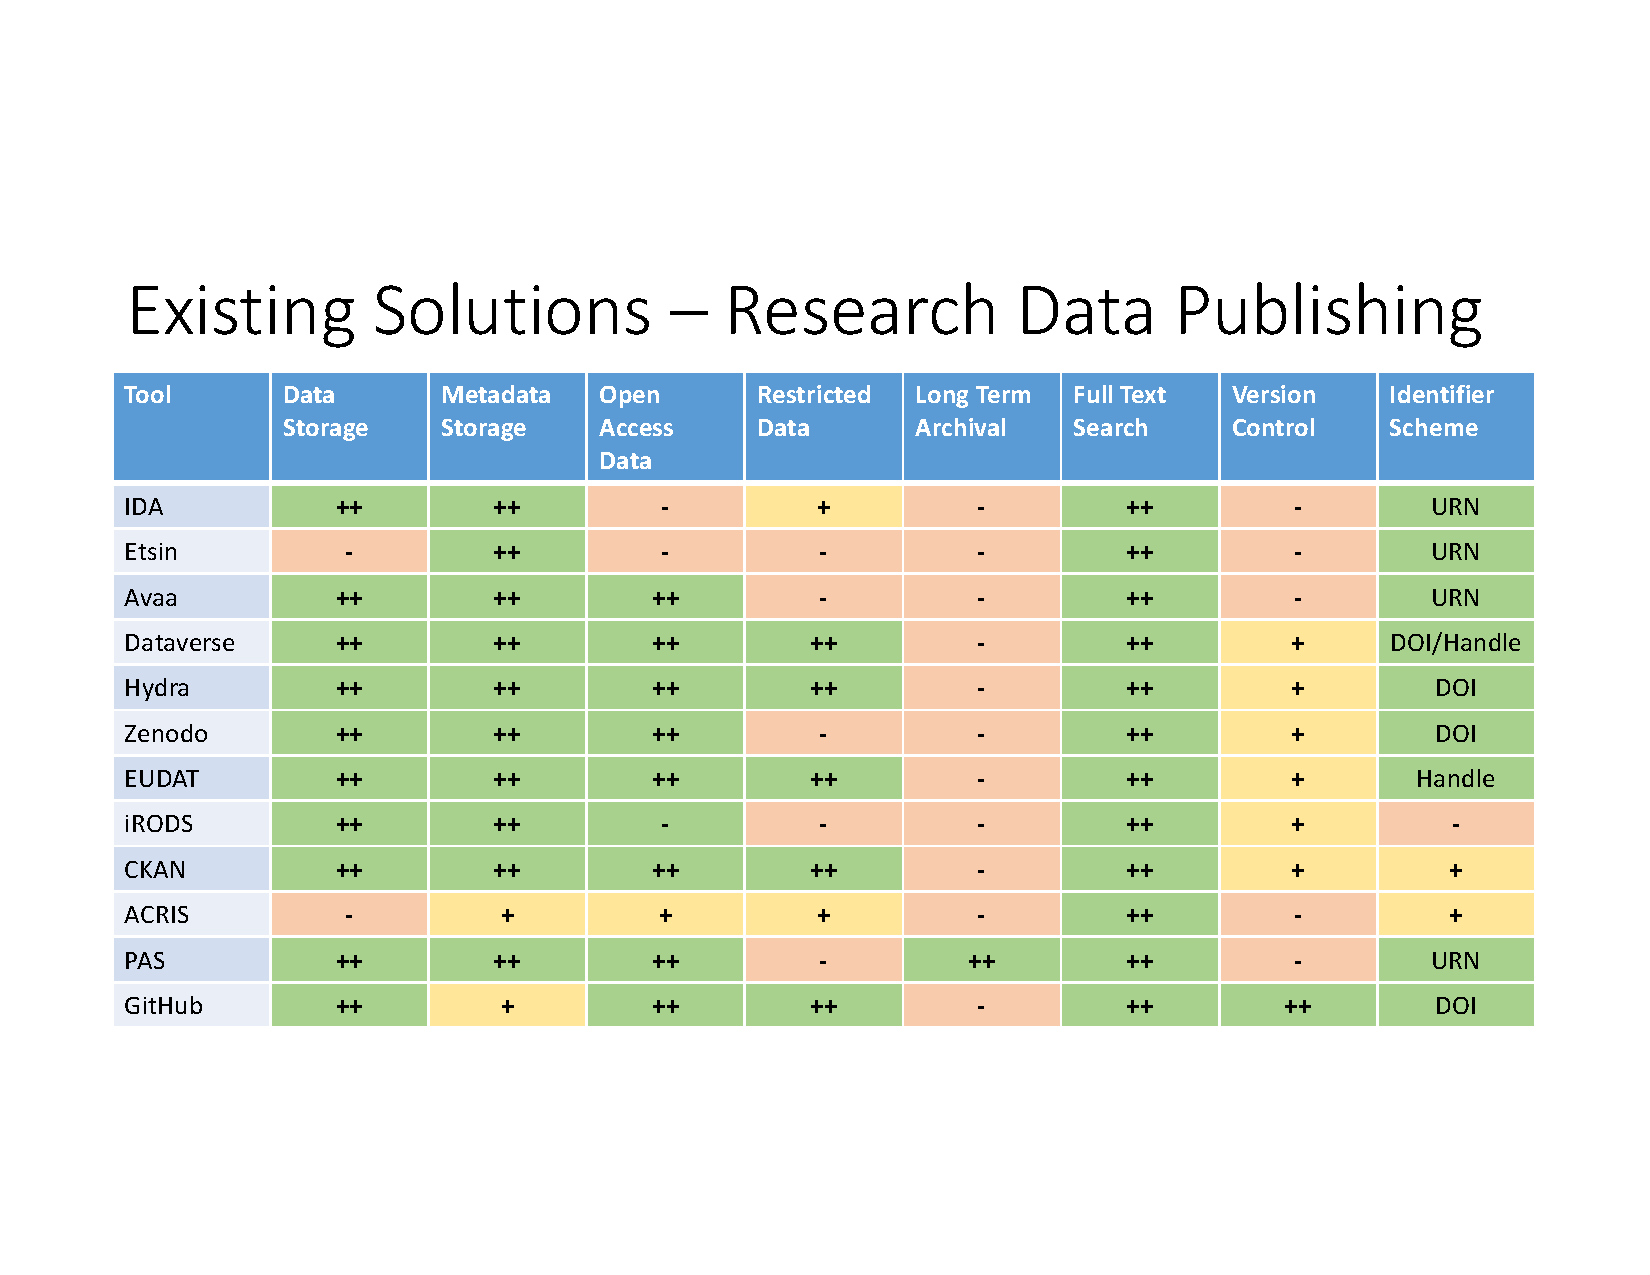
\includegraphics[width=\textwidth]{images/publishing}
    \end{centering}
    \caption{A placeholder for the latex table}
    \label{fig:solutions}
\end{sidewaysfigure}
\fi

Research data publishing is the end goal of research data management, and
Table \ref{table:management} shows the same tools compared previously in
the context of research data publishing being compared in the light
of research data management during the research process. Table
\ref{table:management_features} explains the features that were
explored from the research data management angle.

\captionof{table}{The features being compared on Table \ref{table:management}}
\addtocounter{table}{-1}
\label{table:management_features}
    \begin{tabularx}{\textwidth}{| >{\raggedright}p{3cm} | X |}
    \hline
    \textbf{Feature} & \textbf{Explanation} \\
    \hline
    \rowcolor{Gray}
    File Sharing With Partners    & The basis of collaboration is sharing results and in this
                                    context it means that the solution enables files to be
                                    shared using the system - this also implies that the files
                                    can be stored there for personal use\\
    \hline
    File Editing With Partners & For collaboration just sharing files might not be enough, and
                                 the files should be able to be edited instead of always uploading
                                 new versions to the system\\
    \hline
    \rowcolor{Gray}
    Workflow Sharing    &  The research workflows in some fields of science are highly automated
                           and sharing those would save a lot of time for collaborators and the person
                           sharing them assuming he or she had to return to that workflow later\\
    \hline
    Comments On Files    & Commenting on others' work makes collaboration easier\\
    \hline
    \rowcolor{Gray}
    Web Interface          & A system implements this feature if it has an interface online that
                             can be accessed from anywhere so that the research data is readily
                             accessible\\
    \hline
    Command Line Interface    & A system implements a command line interface if the users can access
                                their research data using technologies like SSH\\
    \hline
    \rowcolor{Gray}
    Desktop Interface       & A system implements a desktop interface if it offers software that the
                              users can install on their personal machines or it integrates to the
                              file system on the user's machine\\
    \hline
    Integrated Data Collection    & Integrated data collection means that tools that collect research
                                    data can be integrated to the solution such that the research data
                                    is collected and put into the systems automatically\\
    \hline
\end{tabularx}

\begin{sidewaystable}
    \caption{Existing solutions in light of research data management}
    \label{table:management}
    \resizebox{\textwidth}{!}{
        \renewcommand{\arraystretch}{2.0}
        \begin{tabular}{| l | c |c | c | c | c | c | c | c | c |}
            \cline{3-10}\cline{1-1}
            \rowcolor{top-level-blue}
            \vspace{1 mm}
            \textbf{Tool} &\cellcolor{white}& \textbf{\vtop{\hbox{\strut File Sharing}\hbox{\strut With Partners}}} & \textbf{\vtop{\hbox{\strut File Editing}\hbox{\strut  With Partners}}} & \textbf{Workflow Sharing} & \textbf{Comments On Files} & \textbf{Web Interface} & \textbf{\vtop{\hbox{\strut Command Line}\hbox{\strut Interface}}} & \textbf{Desktop Interface} & \textbf{\vtop{\hbox{\strut Integrated}\hbox{\strut Data Collection}}} \\
            \cline{3-10}\cline{1-1}
            \cellcolor{first-column-blue}IDA         && \cellcolor{green}++ & \cellcolor{green}++ & \cellcolor{red}-  & \cellcolor{yellow}+  & \cellcolor{green}++  &  \cellcolor{green}++ & \cellcolor{green}++  & \cellcolor{yellow}+ \\
            \cline{3-10}\cline{1-1}
            \cellcolor{first-column-blue}Etsin       && \cellcolor{red}-  & \cellcolor{red}- & \cellcolor{red}-  & \cellcolor{red}-  & \cellcolor{green}++  &  \cellcolor{green}++ & \cellcolor{red}-  & \cellcolor{red}- \\
            \cline{3-10}\cline{1-1}
            \cellcolor{first-column-blue}Avaa        && \cellcolor{green}++ & \cellcolor{red}- & \cellcolor{red}- & \cellcolor{red}-  & \cellcolor{green}++  &  \cellcolor{green}++ & \cellcolor{red}-  & \cellcolor{red}- \\
            \cline{3-10}\cline{1-1}
            \cellcolor{first-column-blue}Dataverse   && \cellcolor{green}++ & \cellcolor{red}- & \cellcolor{red}-  & \cellcolor{yellow}+ & \cellcolor{green}++  &  \cellcolor{green}++ & \cellcolor{red}-  & \cellcolor{red}- \\
            \cline{3-10}\cline{1-1}
            \cellcolor{first-column-blue}Hydra       && \cellcolor{green}++ & \cellcolor{red}- & \cellcolor{red}- & \cellcolor{yellow}+ & \cellcolor{green}++  &  \cellcolor{green}++ & \cellcolor{red}-  & \cellcolor{red}- \\
            \cline{3-10}\cline{1-1}
            \cellcolor{first-column-blue}Zenodo      && \cellcolor{green}++ & \cellcolor{red}- & \cellcolor{red}- & \cellcolor{yellow}+  & \cellcolor{green}++  &  \cellcolor{green}++ & \cellcolor{red}-  & \cellcolor{red}- \\
            \cline{3-10}\cline{1-1}
            \cellcolor{first-column-blue}EUDAT       && \cellcolor{green}++ & \cellcolor{green}++ & \cellcolor{red}- & \cellcolor{yellow}+  & \cellcolor{green}++  &  \cellcolor{green}++ & \cellcolor{green}++  & \cellcolor{red}- \\
            \cline{3-10}\cline{1-1}
            \cellcolor{first-column-blue}iRODS       && \cellcolor{green}++ & \cellcolor{green}++ & \cellcolor{red}-  & \cellcolor{yellow}+  & \cellcolor{green}++  &  \cellcolor{green}++ & \cellcolor{green}++  & \cellcolor{green}++ \\
            \cline{3-10}\cline{1-1}
            \cellcolor{first-column-blue}CKAN        && \cellcolor{green}++ & \cellcolor{red}- & \cellcolor{red}- & \cellcolor{yellow}+ & \cellcolor{green}++  &  \cellcolor{green}++ & \cellcolor{red}-  & \cellcolor{red}- \\
            \cline{3-10}\cline{1-1}
            \cellcolor{first-column-blue}ACRIS       && \cellcolor{green}++  & \cellcolor{red}-  & \cellcolor{red}-  & \cellcolor{red}-  & \cellcolor{green}++  &  \cellcolor{green}++ & \cellcolor{red}-  & \cellcolor{red}- \\
            \cline{3-10}\cline{1-1}
            \cellcolor{first-column-blue}PAS         && \cellcolor{green}++ & \cellcolor{red}- & \cellcolor{red}- & \cellcolor{red}-  & \cellcolor{green}++ &  \cellcolor{green}++ & \cellcolor{red}-  & \cellcolor{red}- \\
            \cline{3-10}\cline{1-1}
            \cellcolor{first-column-blue}GitHub      && \cellcolor{green}++ & \cellcolor{green}++  & \cellcolor{red}- & \cellcolor{green}++ & \cellcolor{green}++  &  \cellcolor{green}++ & \cellcolor{green}++ & \cellcolor{red}- \\
            \cline{3-10}\cline{1-1}
        \end{tabular}
    }
\end{sidewaystable}

\iffalse
\begin{sidewaysfigure}
    \begin{centering}
        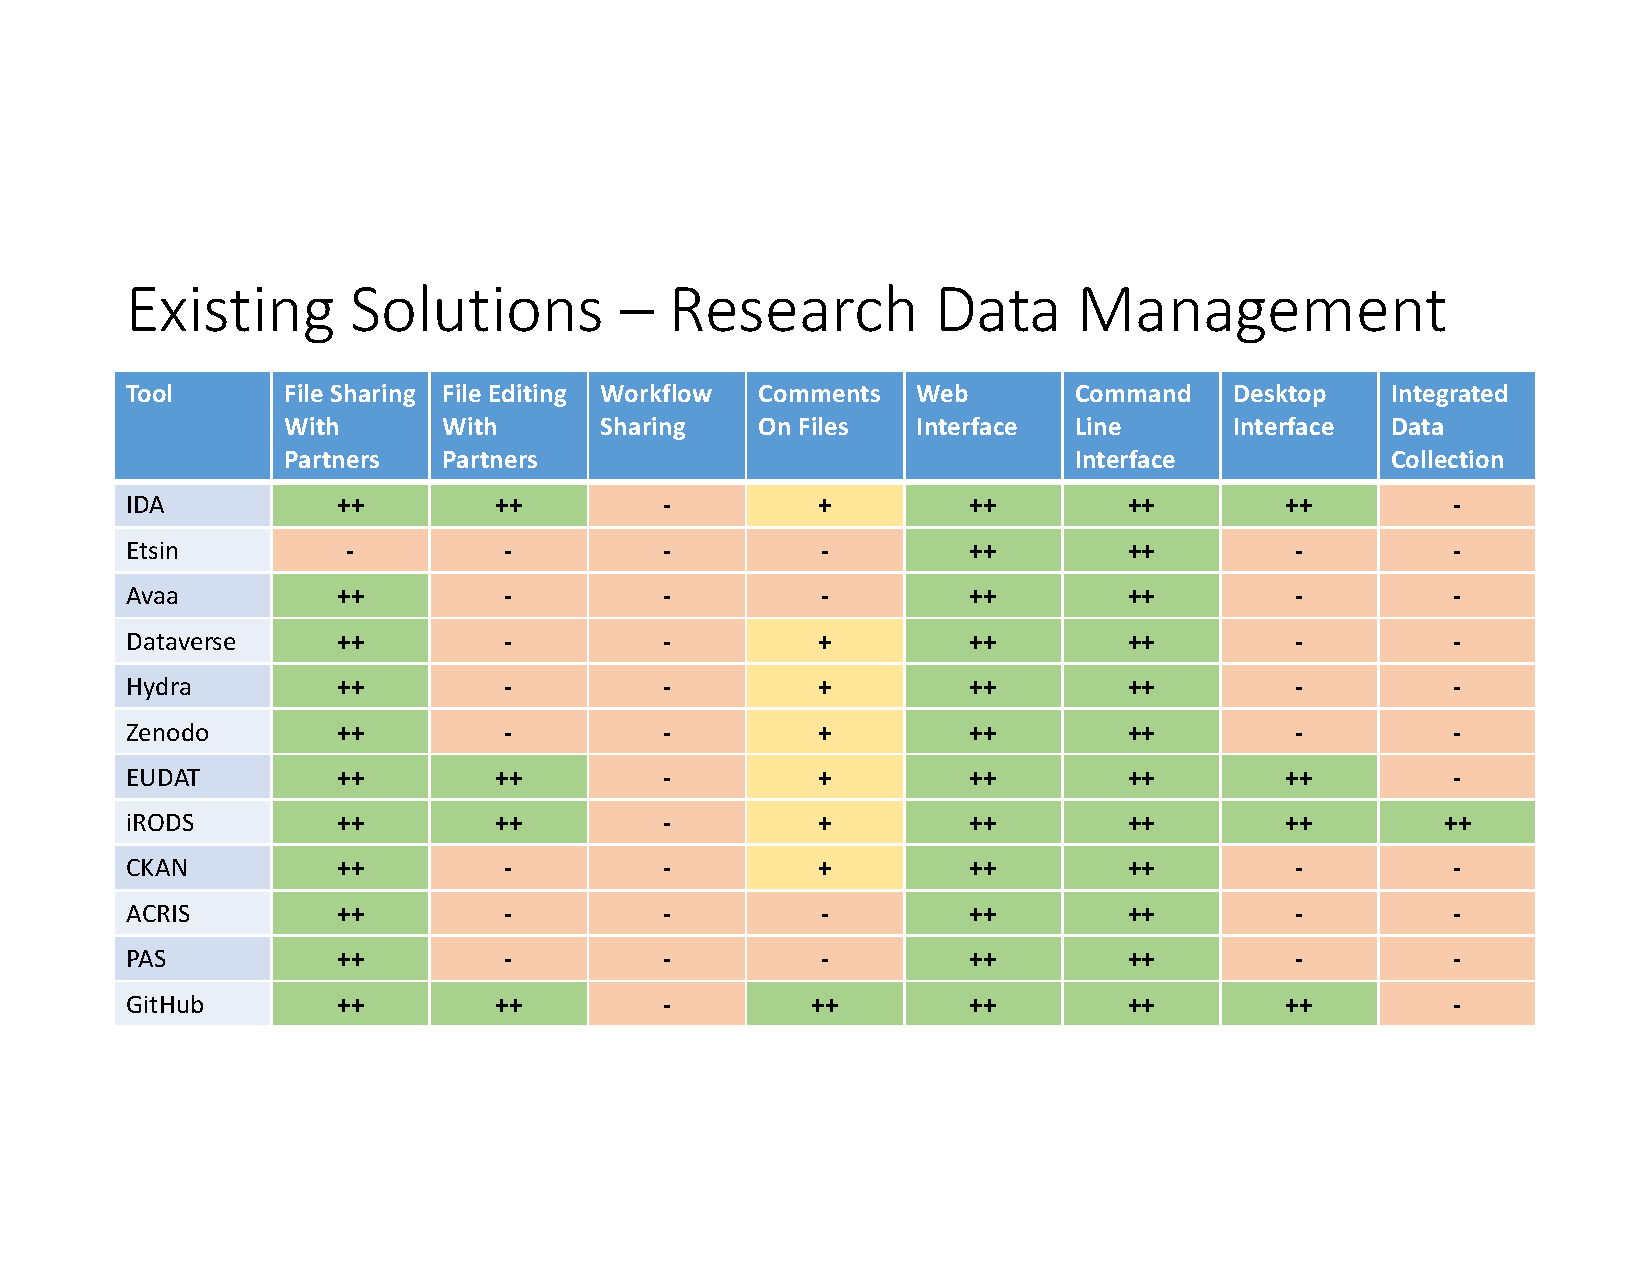
\includegraphics[width=\textwidth]{images/management}
    \end{centering}
    \caption{A placeholder for the latex table}
    \label{fig:management}
\end{sidewaysfigure}
\fi

The same tools that are suitable for research data publishing are not
necessarily right for research data management and vice versa. iRODS, IDA
and the B2Drop side of the EUDAT service offer dedicated services to share research data during
the research process and manage it in a centralized service. GitHub is a
collaborative tool for projects around programming.

The tools that work well for research data publishing lack many important
features that research data management and research collaboration, such
as file editing and proper commenting functionality on file. Research workflows
cannot be stored or shared with any of the tools, which is not surprising - the
definition of a workflow varies a lot between disciplines and it is not a
requirement for many.

The user tests and interviews also show that the research management ways
of researchers could be much better. Research data management is learned
by doing and from peers and the awareness of good practices and tools for
research data management is low. Good practices and tools should be taught to
the researchers creating and managing the research data.

When looking at the existing solutions through both the context of research
data management and publishing it is clear that a big problem is that there
is not a solution that would handle the entire lifecycle of the data from
creation to publishing. Research data sharing and managing should not be considered
separately from research data management. Without management, there can not be
effective sharing or publishing and without sharing or publishing there is no
need for management. Many universities, Aalto University included, have
implemented neither managing or publishing research data tools in a centralized
way. The lack of dedicated research data management
infrastructure also affects the training and knowledge of research data
management and tools in the sense that if there is no infrastructure to
leverage there is no way to teach institutional best practices.

This thesis set out to answer two research questions. Firstly, how research
data can be shared and published using modern tools and how these tools work
in practice? Secondly, what are the non technical matters that affect sharing
and publishing research data? To answer the first question we have found, presented and tested existing software
solutions for research data publishing and sharing. Through user testing and technical benchmarking
we have concluded that the user experience of these solutions could be enhanced to make research data
sharing and publishing easier, but the solutions do serve their purpose and can be used
to share and publish research data. Additionally, the lack of tools to manage research data
during the research process makes publishing and sharing research data harder. As for the second question, we have
concluded using user interviews and user tests that the lack of culture, incentives
and know-how about research data sharing, publishing and management is a major
barrier to publishing and sharing research data.

Following these conclusions we have presented steps to make research data publishing
and sharing prevalent in the field of science. In order to make the tools
for sharing and publishing research data better, holistic solutions that combine
research data management, publishing and sharing should be implemented. Solving
the non technical problems of research data management, sharing and publishing
starts from proving the benefits of sharing and publishing research data and
from providing education and incentives for researchers.


% Appendices go here
% ------------------------------------------------------------------
% If you do not have appendices, comment out the following lines
%\startchapright
\appendix
\chapter{First appendix}
\label{chapter:first-appendix}

This is the first appendix. You could put some test images or verbose data in an
appendix, if there is too much data to fit in the actual text nicely.

For now, the Aalto logo variants are shown in Figure~\ref{fig:aaltologo}.

\begin{figure}
\begin{center}
 \begin{subfigure}[b]{\textwidth}
  {\selectlanguage{english}\AaltoLogoSmall{1}{!}{aaltoBlue}}
  \caption{In English}
 \end{subfigure}
 \begin{subfigure}[b]{\textwidth}
  {\selectlanguage{finnish}\AaltoLogoSmall{1}{''}{aaltoRed}}
  \caption{Suomeksi}
 \end{subfigure}
 \begin{subfigure}[b]{\textwidth}
  {\selectlanguage{swedish}\AaltoLogoSmall{1}{?}{aaltoYellow}}
  \caption{P\r{a} svenska}
 \end{subfigure}
\caption{Aalto logo variants}
\label{fig:aaltologo}
\end{center}
\end{figure}


% Load the bibliographic references
% ------------------------------------------------------------------
\startchapright
\phantomsection
\addcontentsline{toc}{chapter}{Bibliography}
% You can use several .bib files:
% \bibliography{thesis_sources,ietf_sources}
\bibliography{sources}

% End of document!
% ------------------------------------------------------------------
% The LastPage package automatically places a label on the last page.
% That works better than placing a label here manually, because the
% label might not go to the actual last page, if LaTeX needs to place
% floats (that is, figures, tables, and such) to the end of the 
% document.
\end{document}
